% IEEEAerospace2012.cls requires the following packages: times, rawfonts, oldfont, geometry
\documentclass[twocolumn,letterpaper]{IEEEAerospaceCLS}  % only supports two-column, letterpaper format

% The next line gives some packages you may find useful for your paper--these are not required though.
%\usepackage[]{graphicx,float,latexsym,amssymb,amsfonts,amsmath,amstext,times,psfig}
% NOTE: The .cls file is now compatible with amsmath!!!

\usepackage{siunitx}      % Use for scientific notation.
\usepackage{float}        % Use to not have figures placed in random locations.
\usepackage[]{graphicx}   % We use this package in this document.
\usepackage[font=footnotesize,labelfont=bf,textfont=bf]{caption}
\usepackage{subcaption}   % neue subfigure-Umgebung %% should probably not be used with memoir: generates warning
\usepackage[nolist,nohyperlinks]{acronym} % Use this for acronyms, unlisted.

% New commands.
\newcommand{\ignore}[1]{}                  % {} empty inside = %% comment.
\newcommand{\refFig}[1]{{Figure}~\ref{#1}} % Command for figure reference.
\newcommand{\refTab}[1]{{Table}~\ref{#1}}  % Command for table reference.

% Renew commands.
\renewcommand\thefootnote{{(\alph{footnote})}} % footnote formatting and colors

% Define common figure sizes for subfigures -> redefined in each environment
\newlength{\subfigureWidth}
\setlength{\subfigureWidth}{0.24\textwidth}
\newlength{\graphicsHeight}
\setlength{\graphicsHeight}{25mm}

\begin{acronym}
  \acro{DFKI}{German Research Center for Artificial Intelligence}
  \acro{EOL}{End of Life}
  \acro{IL}{InnerLeg}
  \acro{MRS}{Multi-Robot System}
  \acro{OL}{OuterLeg}
  \acro{PLI}{Payload Item}
  \acro{RA}{Robotic Arm}
  \acro{RIC}{Robotics Innovation Center}
  \acro{SA}{Solar Array}
  %\acrodefplural{SA}[SAs]{Solar Arrays}
  \acro{TRL}{Technology Readiness Level}
  \acro{WD}{WheelDrive}
  \acro{WS}{WheelSteering}
\end{acronym}

\begin{document}
\title{Using a Rover's Active Suspension System as a 2-Axis Solar Tracker Mechanism}

% Alternative titles:
%   1. Daily Solar Array Reconfiguration with the SherpaTT Rover Active Suspension System for Long Traverses
%   2. Extending Rover Traverse Coverage with the SherpaTT Active Suspension System for Daily Solar Array Reconfiguration
%   3. Using the SherpaTT Active Suspension for Daily Optimization of Solar Array Configuration
%   4. The SherpaTT Rover's Active Suspension System as a Mechanism for Daily Optimization of Solar Array Configuration
%   5. Using the SherpaTT Active Suspension System for Daily Optimization of Rover Solar Array Configuration
%   6. The SherpaTT Rover Active Suspension System as a Mechanism for Daily Solar Array Optimization
%   7. Mars Traverse Distance Gains Using a Rover's Active Suspension System as a 2-Axis Solar Tracker Mechanism
\author{%
Georges L. J. Labrèche\\
Georges.Labreche@gmail.com
\and
Florian Cordes\\
DFKI Robotics Innovation Center\\
Robert-Hooke-Straße 1\\
28359 Bremen, Germany\\
Florian.Cordes@dfki.de
}

\maketitle

\thispagestyle{plain}
\pagestyle{plain}


\begin{abstract}
The SherpaTT rover is prepared for further autonomous long distance traverses in terrain akin to the Martian environment. However, it features a fueled power generator which cannot be employed in extra-terrestial scenarios. As the rover is meant to approach a higher technology readiness level, a photovoltaic power subsystem is proposed to guide future design iterations. This paper presents the solar array sizing, design, and integration processes considered for two Martian mission sites: Iani Chaos at \SI{2}{\degree}S and Ismenius Cavus at \SI{34}{\degree}N. An alternative use case for the active suspension system is presented so that the proposed solar arrays may be inclined and oriented into power generating configurations that are more favorable than those achieved with passive suspension rovers. This results in traverse gains of up to \SI{34}{\percent} and \SI{25}{\percent} for clear days at Iani Chaos and Ismenius Cavus, respectively.
\end{abstract}


% Table of content is not needed.
% \tableofcontents

%%%%%%%%%%%%%%%%%%%%%%%%%%%%%%%%%%%%%%
\section{Introduction}
%%%%%%%%%%%%%%%%%%%%%%%%%%%%%%%%%%%%%%
The exploration rover SherpaTT has a total mass of approximately \SI{206}{\kilo\gram} and the legs as well as the \ac{RA} weigh about \SI{25}{\kilo\gram} each. The wheeled-leg active suspension system allows the rover to assume different poses with varying inertial moments. The rover is one of many systems comprising a \ac{MRS} developed at the \ac{DFKI}'s \ac{RIC}.

The rover has undergone several field trial campaigns, particularly with a Mars analogue terrain field deployment in Utah, USA, where a logistics chain for sample return was evaluated. The rover's versatility has been demonstrated through a multitude of tasks such as assembling surface deployable payloads and using its \ac{RA} for soil sampling with modular \ac{PLI} sampling devices \cite{Cordes2018b}.

\begin{figure}[h]
  \centering
  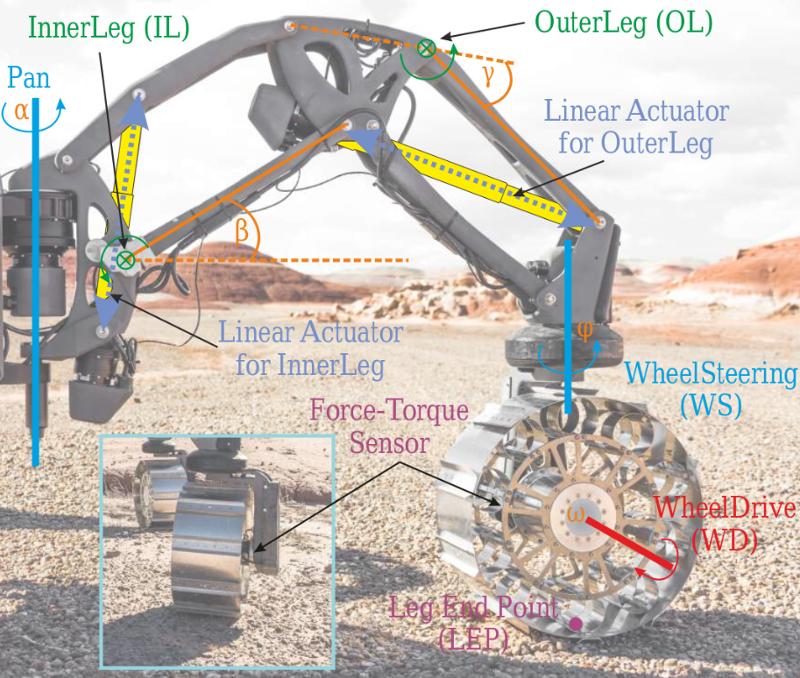
\includegraphics[width=2.9in]{figures/images/sherpatt-actively-articulated-suspension-sytem.png}\\
  \caption{Description of DoF present in SherpaTT’s
suspension system and placement of force-torque sensor}
  \label{fig:sherpatt-actively-articulated-suspension-system}
\end{figure}

The actively articulated suspension system consists of four wheeled-legs with a total of 20 motors. The distribution of motors across a single leg is shown in \refFig{fig:sherpatt-actively-articulated-suspension-system}. Each leg is equipped with three suspension motors and two drive motors. The suspension motors are responsible for Pan, \ac{IL}, and \ac{OL} revolute joint rotations whereas the drive motors are responsible for \ac{WS} and \ac{WD}.

The rover has been deployed in several field experiments where it was put under test within natural and unstructured Mars analogue terrain with respect to general morphology and geology. The rover displayed the ability to cope with natural terrain and to fulfill the task of being an exploration and sampling rover. Further development is required on its electrical power subsystem if it is to operate in long term missions. This paper explores \ac{SA} configurations for the a Mars environment in order to guide future design iterations to navigate the topography of this planetary surface. The constraints imposed from the active suspension system with flexible footprints and varying heights of structural parts of the legs are considered in the design phase.

Initial \ac{SA} sizing requirements are derived from Mars mission sites, Iani Chaos and Ismenius Cavus, that impose energy storage and consumption constraints based on available daily insolations. The design is driven by the use the rover's active suspension system as a 2-axis solar tracking mechanism, enabling daily reconfiguration of the \ac{SA} surface inclination and orientation angles. An alternative use of the wheeled leg system is thus presented for a use case that goes beyond the scenario of negotiating complex terrains such as steep slopes. Specifically, the findings demonstrate traverse and mass reductions gains that are obtained with a suspension system driven inclination and orientation capable \ac{SA} surface when compared to a horizontal configuration.

Past research on active suspension systems are restricted to analyzing benefits with respect to traversing challenging topographies. Studying how this system can be used for other mission planning elements broadens the field of research.

%%%%%%%%%%%%%%%%%%%%%%%%%%%%%%%%%%%%%%%%%%%
\section{Power Budget}
%%%%%%%%%%%%%%%%%%%%%%%%%%%%%%%%%%%%%%%%%%%

Large inclination angles are typically preferred with respect to increased insolation for a sun-facing surface. However, constraints on the rover's active suspension system impose a limit on the achievable body pitch angle. Body pitch commands of up to \SI{10}{\degree} are experimentally evaluated during steep slope climbing in \cite{Cordes2018a}. Modeling higher pitch angles resulted in poor wheel-ground contact angle due to the \ac{WS} axis having the same tilt as the rover's body. The attainable tilt is thus restricted resulting in a maximum \ac{SA} surface inclination angle of $\beta = \SI{10}{\degree}$.

\begin{table}[h]
  \footnotesize
  \centering
  \caption{Worst and best case daily insolations at Iani Chaos.}
  \label{tab:insolation-iani-chaos-clear-and-dusty-days}
  \begin{tabular}{c|c|c|c|c|c|c|c|c|}
    \cline{2-9}
    \multicolumn{1}{l|}{} & \multicolumn{4}{c|}{Worst Case} & \multicolumn{4}{c|}{Best Case} \\ \hline
    \multicolumn{1}{|c|}{$\tau$} & $L_{s}$ & $H_{h}$ & $H_{\beta}$ & $gain$ & $L_{s}$ & $H_{h}$ & $H_{\beta}$ & $gain$ \\ \hline
    \multicolumn{1}{|c|}{0.1} & 80 & 3232 & 3721 & 15.13 & 221 & 5076 & 5695 & 12.19 \\ \hline
    \multicolumn{1}{|c|}{0.4} & 81 & 2909 & 3166 & 8.85 & 218 & 4613 & 4933 & 6.93 \\ \hline
    \multicolumn{1}{|c|}{0.5} & 81 & 2812 & 3025 & 7.58 & 218 & 4473 & 4736 & 5.89 \\ \hline
    \multicolumn{1}{|c|}{1.0} & 82 & 2391 & 2479 & 3.67 & 214 & 3855 & 3959 & 2.69 \\ \hline
    \multicolumn{1}{|c|}{1.5} & 82 & 2087 & 2125 & 1.81 & 213 & 3403 & 3444 & 1.19 \\ \hline
  \end{tabular}
\end{table}


\refTab{tab:insolation-iani-chaos-clear-and-dusty-days} and \refTab{tab:insolation-ismenius-cavus-clear-and-dusty-days} present the best and worst case daily insolations $H_{h}$, on horizontal \ac{SA} surface, compared to those obtained with $H_{\beta}$, on an inclined sun-facing \ac{SA} surface. Optical depths $\tau$ for clear to dusty days are evaluated with the daily insolations expressed in \si{Wh.m^{-2}} and the gains in percentage. The solar insolation values are taken from \cite{Labreche2020}.

\begin{table}[h]
  \footnotesize
  \centering
  \caption{Worst and best case daily insolations at Ismenius Cavus.}
  \label{tab:insolation-ismenius-cavus-clear-and-dusty-days}
  \begin{tabular}{c|c|c|c|c|c|c|c|c|}
    \cline{2-9}
    \multicolumn{1}{l|}{} & \multicolumn{4}{c|}{Worst Case} & \multicolumn{4}{c|}{Best Case} \\ \hline
    \multicolumn{1}{|c|}{$\tau$} & $L_{s}$ & $H_{h}$ & $H_{\beta}$ & $gain$ & $L_{s}$ & $H_{h}$ & $H_{\beta}$ & $gain$ \\ \hline
    \multicolumn{1}{|c|}{0.1} & 274 & 2102 & 2762 & 31.42 & 127 & 4421 & 4925 & 11.40 \\ \hline
    \multicolumn{1}{|c|}{0.4} & 273 & 1752 & 2030 & 15.85 & 125 & 4028 & 4289 & 6.49 \\ \hline
    \multicolumn{1}{|c|}{0.5} & 273 & 1655 & 1869 & 12.93 & 124 & 3908 & 4122 & 5.48 \\ \hline
    \multicolumn{1}{|c|}{1.0} & 273 & 1284 & 1345 & 4.75 & 121 & 3378 & 3461 & 2.44 \\ \hline
    \multicolumn{1}{|c|}{1.5} & 273 & 1045 & 1061 & 1.57 & 120 & 2945 & 2973 & 0.96 \\ \hline
  \end{tabular}
\end{table}


Gains obtained in daily insolation with an inclined surface are more pronounced for sites further away from the equator. For a typical optical depth of $\tau = 0.4$, the average daily insolation gain on the inclined surface is approximately \SI{7}{\percent} at Iani Chaos and \SI{9}{\percent} at Ismenius Cavus.
Due to the mostly diffuse composition of solar irradiance at higher optical depths, inclined surfaces become irrelevant during global dust storms. For $\tau \geq 2$, gains in daily insolation become negligible at both sites.

As a prerequisite to \ac{SA} sizing, power budgets are defined for hibernation and flat terrain traverse reference Sols. These are presented in \refTab{tab:hibernation-sol-power-budget} and \refTab{tab:worst-case-traverse-sol-power-budget}. Hibernation power draws are identical during day and nighttime so the hibernation reference Sol does not have a best or worse case Sol with respect to available sunlight.

\begin{table}[h]
  {\def\arraystretch{1.4} % Extra vertical spacing.
  \footnotesize
  \centering
  \caption{Hibernation Sol power budget.}
  \label{tab:hibernation-sol-power-budget}
  \begin{tabular}{lc|c|c|c|c|}
    \cline{3-6}
     & & \multicolumn{2}{c|}{Iani Chaos} & \multicolumn{2}{c|}{Ismenius Cavus} \\ \hline
    \multicolumn{1}{|l|}{Mode} & P {[}W{]} & t {[}min{]} & E {[}Wh{]} & t {[}min{]} & E {[}Wh{]} \\ \hline
    \multicolumn{1}{|l|}{Day} & 18 & 720 & 216 & 720 & 216 \\ \hline
    \multicolumn{1}{|l|}{Night} & 18 & 720 & 216 & 720 & 216 \\ \hline
    \multicolumn{1}{|r|}{Total} & 36 & 1440 & 432 & 1440 & 432 \\ \hline
    \multicolumn{1}{|r|}{+20\% Margin} & 43 & - & 518 & - & 518 \\ \hline
  \end{tabular}
\end{table}


Durations of daylight dependent modes in the traverse reference Sol are based on the total length of daylight time for worst case daily insolations Sols presented in \refTab{tab:insolation-iani-chaos-clear-and-dusty-days} and \refTab{tab:insolation-ismenius-cavus-clear-and-dusty-days} with $\tau$ factor 1 and $\beta=\SI{10}{\degree}$ for the \ac{SA} surface inclination angle. Propulsion power draws for the rover's flat terrain traverse mode is determined from data collected during the SherpaTT Utah field trial \cite{Cordes2018b}.

\begin{table}[h]
  \footnotesize
  \centering
  \caption{Worst case flat traverse Sol power budget, $\tau$\,=\,1 and $\beta$\,=\,\SI{10}{\degree}.}
  \label{tab:worst-case-traverse-sol-power-budget}
  \begin{tabular}{lc|c|c|c|c|}
    \cline{3-6}
     & & \multicolumn{2}{c|}{\begin{tabular}[c]{@{}c@{}}Iani Chaos\\ $Ls=\SI{81}{\degree}$\end{tabular}} & \multicolumn{2}{c|}{\begin{tabular}[c]{@{}c@{}}Ismenius Cavus\\ $Ls=\SI{273}{\degree}$\end{tabular}} \\ \hline
    \multicolumn{1}{|l|}{Mode} & P {[}W{]} & t {[}min{]} & E {[}Wh{]} & t {[}min{]} & E {[}Wh{]} \\ \hline
    \multicolumn{1}{|l|}{Idle - Day} & 29 & 603 & 291 & 464 & 224 \\ \hline
    \multicolumn{1}{|l|}{Communication} & 52 & 35 & 30 & 35 & 30 \\ \hline
    \multicolumn{1}{|l|}{Traverse} & 113 & 4.8 & 9 & 4.8 & 9 \\ \hline
    \multicolumn{1}{|l|}{Science Stop} & 60 & 60 & 60 & 60 & 60 \\ \hline
    \multicolumn{1}{|l|}{Optimal Pose} & 75 & 12 & 13 & 10 & 13 \\ \hline
    \multicolumn{1}{|l|}{Idle - Night} & 20 & 242 & 242 & 866 & 289 \\ \hline
    \multicolumn{1}{|r|}{Total} & 349 & 1440 & 646 & 1440 & 625 \\ \hline
    \multicolumn{1}{|r|}{+20\% Margin} & 419 & - & 775 & - & 750 \\ \hline
  \end{tabular}
\end{table}


The \textit{Optimal Pose} mode in \refTab{tab:worst-case-traverse-sol-power-budget} consists of using the rover's active suspension system to reconfigure the \ac{SA} surface orientation and inclination so that daily insolation is maximized on the following Sol. In this manner, the suspension system undertakes the role of a 2-axis solar tracking mechanism.

%%%%%%%%%%%%%%%%%%%%%%%%%%%%%%%%%%%%%%%%%%%
\section{Solar Array Sizing}
%%%%%%%%%%%%%%%%%%%%%%%%%%%%%%%%%%%%%%%%%%%

The solar cell coverage area $A$ is expressed as:

\begin{equation}
  \label{eq:solar_cell_coverage_area}
  A = \frac{E}{\eta \cdot H \cdot PR}
\end{equation}

where $E$ is the rover's energy requirement, $\eta$ is the solar cell efficiency, $H$ is the daily insolation, and $PR$ is the solar cell performance ratio. An initial \ac{SA} sizing is determined with $H_{\beta}$ from \refTab{tab:insolation-iani-chaos-clear-and-dusty-days} and \refTab{tab:insolation-ismenius-cavus-clear-and-dusty-days} as well as $E$ from \refTab{tab:worst-case-traverse-sol-power-budget} for the worst case daily insolation at $\tau$ factor 1. \ac{EOL} values for $PR$ and $\eta$ are determined in \cite{Labreche2020}:

\begin{itemize}
  \item [(1)] $H$\,$=$\,\SI{2479}{Wh.m^{-2}} and $E$\,$=$\,\SI{775}{\watt\hour} at Iani Chaos.
  \item [(2)] $H$\,$=$\,\SI{1345}{Wh.m^{-2}} and $E$\,$=$\,\SI{750}{\watt\hour} at Ismenius Cavus.
  \item [(3)] $PR_{EOL}$\,$=$\,0.62.
  \item [(4)] $\eta_{EOL}$\,$=$\,0.22.
\end{itemize}

Furthermore, the solar cell packing efficiency is assumed at \SI{85}{\percent}, the \ac{SA} surface density at \SI{3.7}{kg.m^{-2}}, and the average slippage at \SI{15}{\percent} when traversing a flat terrains for any given distance. Traversing is constrained to daylight hours and it is assumed that on average traversing only occurs every third Sol.

At Iani Chaos, the required \ac{SA} area is \SI{2.7}{m^{2}} and the mass 9.95 \si{\kilo\gram}. \ac{SA} surface inclination of \SI{10}{\degree} with a daily sun-facing reorientation results in a \ac{SA} size decrease of \SI{3.9}{\percent} when compared against a horizontal surface configuration. The maximum flat traverse distance achievable over the course of a Martian year is increased by \SI{13.22}{\percent} from \SI{42.43}{\kilo\meter} to \SI{48.04}{\kilo\meter} with $\tau$ factor 1 during global dust storm season and 0.4 otherwise. At Ismenius Cavus, the required \ac{SA} area is \SI{4.8}{m^{2}}, its mass 17.8 \si{\kilo\gram}, and a \SI{4.6}{\percent} \ac{SA} size decrease is achieved. The maximum flat traverse distance achievable over the course of a Martian year is increased by \SI{2.13}{\percent} from \SI{63.05}{\kilo\meter} to \SI{64.39}{\kilo\meter}.

The traverse distance gains attributed to \ac{SA} inclination capabilities do not justify taking advantage of the rover's active suspension system for the purpose of increasing solar power generation. This is particularly true at Ismenius Cavus. The savings in \ac{SA} size and mass also leave much to be desired. Furthermore, the large \ac{SA} are problematic in terms of rover integration. This is illustrated in \refFig{fig:sa-area-initial-sizes}.

\begin{figure}[h]
  \centering
  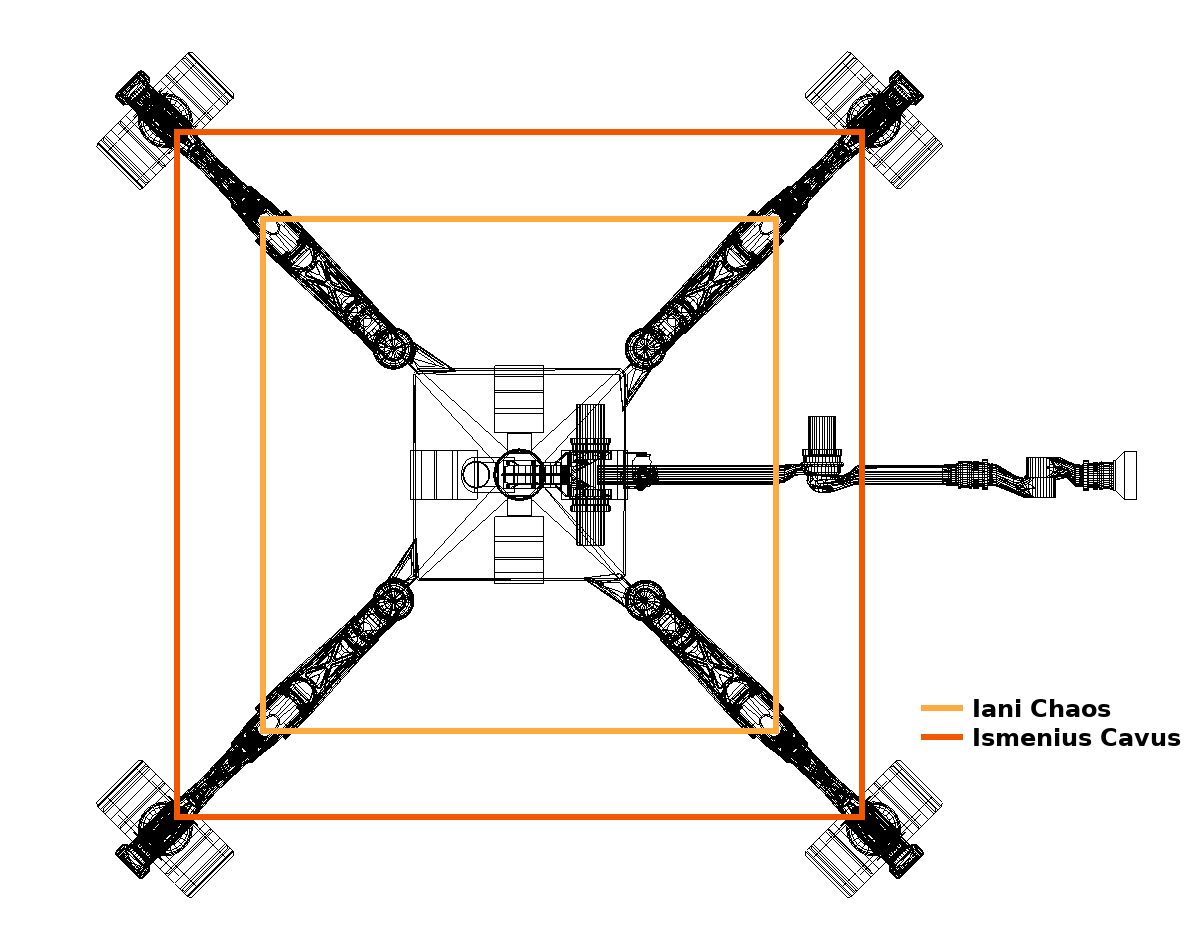
\includegraphics[width=3.25in]{figures/images/sa-area-initial-sizes.png}\\
  \caption{Initial \ac{SA} sizing. The outlined square areas are equivalent to \ac{SA} areas of \SI{2.7}{m^{2}} for Iani Chaos and \SI{4.8}{m^{2}} for Ismenius Cavus.}
  \label{fig:sa-area-initial-sizes}
\end{figure}


To explain the lack of significant gains, the generated \ac{SA} energy and maximum traverse durations are plotted in \refFig{fig:plot:ismenius-cavus-generated-energy-and-max-traverse-durations} for Ismenius Cavus. During clear days at $\tau$ factor 0.4, a ceiling is imposed on the daily maximum traverse durations due to the available daylight time for traversing. The maximum traverse time is already attained with a horizontal \ac{SA}, making an inclined \ac{SA} irrelevant in terms traverse distance gains. As seen in \refFig{fig:plot:sub:ismenius-cavus-max-traverse-durations}, the inclined \ac{SA} is only slightly advantageous during the global dust storm season with a $\tau$ factor of 1.

\begin{figure}[h]
\captionsetup[subfigure]{justification=centering}
  \centering
  \setlength{\subfigureWidth}{0.24\textwidth}
  \setlength{\graphicsHeight}{40mm}
  \begin{subfigure}[t]{\subfigureWidth}
    \centering
    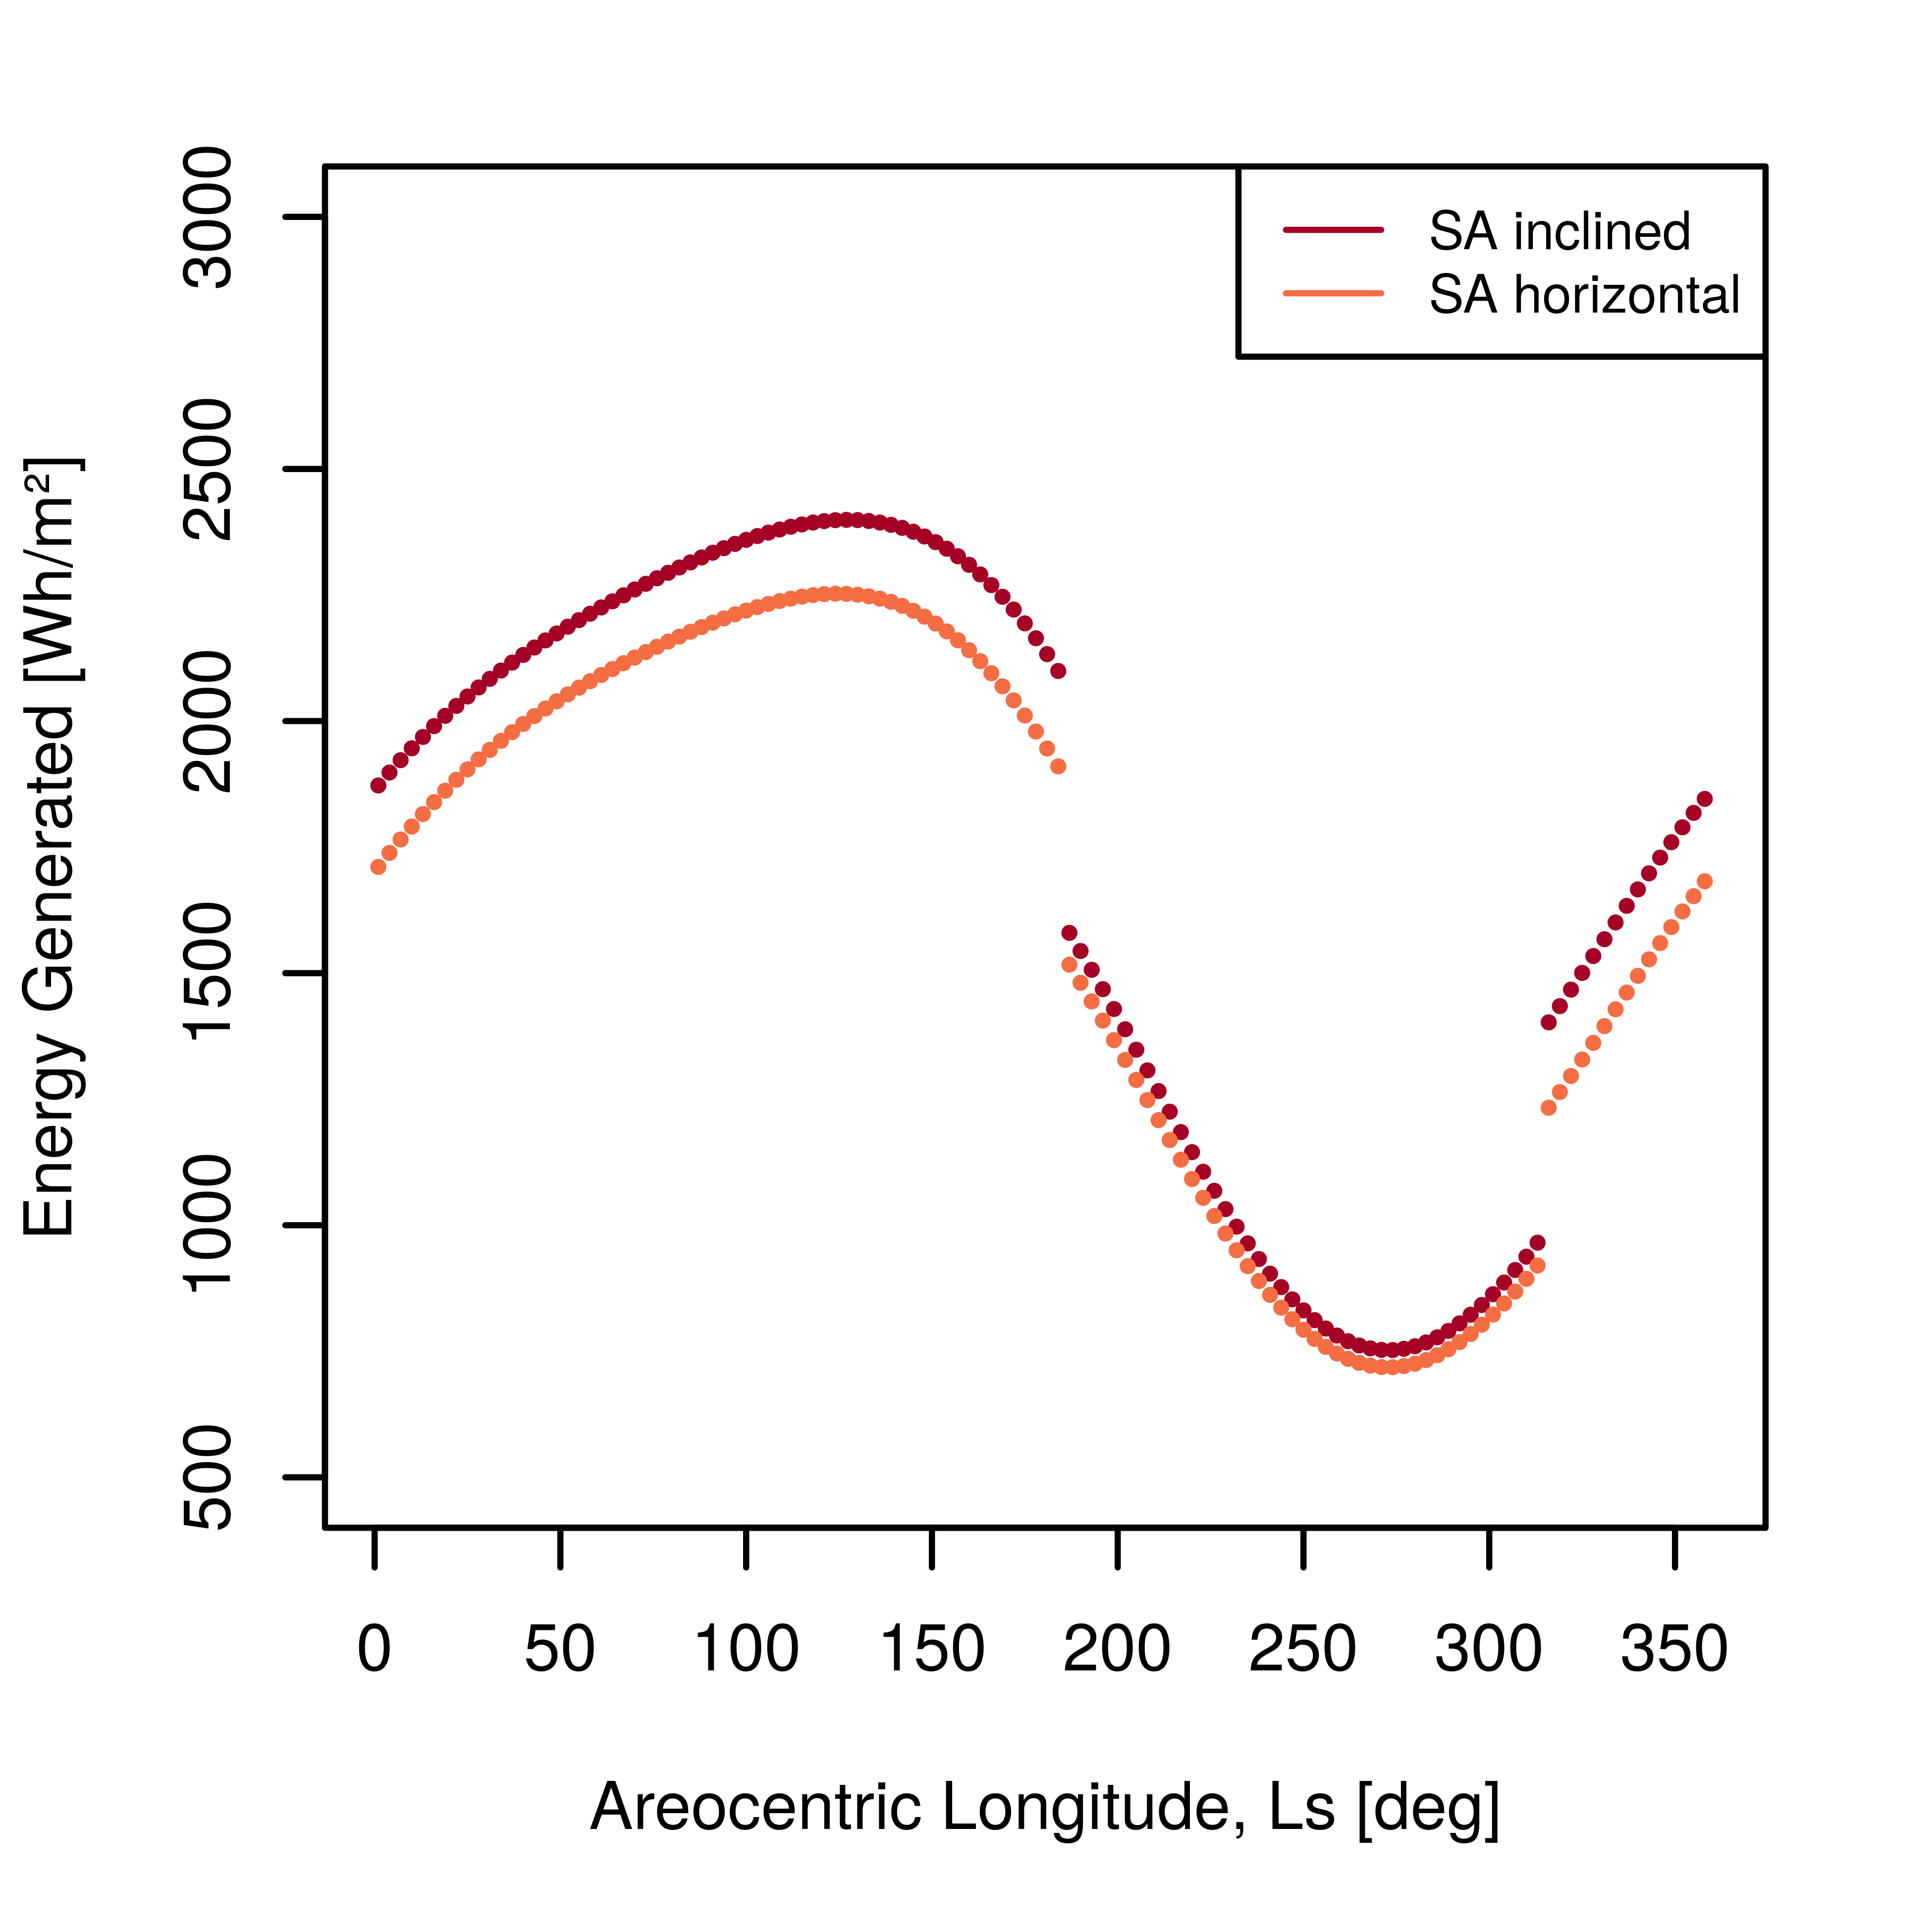
\includegraphics[height=\graphicsHeight]{figures/plots/ismeniuscavus-daily-generated-energy-for-solar-cell-coverage-area-41m2.png}
    \subcaption{Generated Energy}
    \label{fig:plot:sub:ismenius-cavus-generated-energy}
  \end{subfigure}\hfill
  \begin{subfigure}[t]{\subfigureWidth}
    \centering
    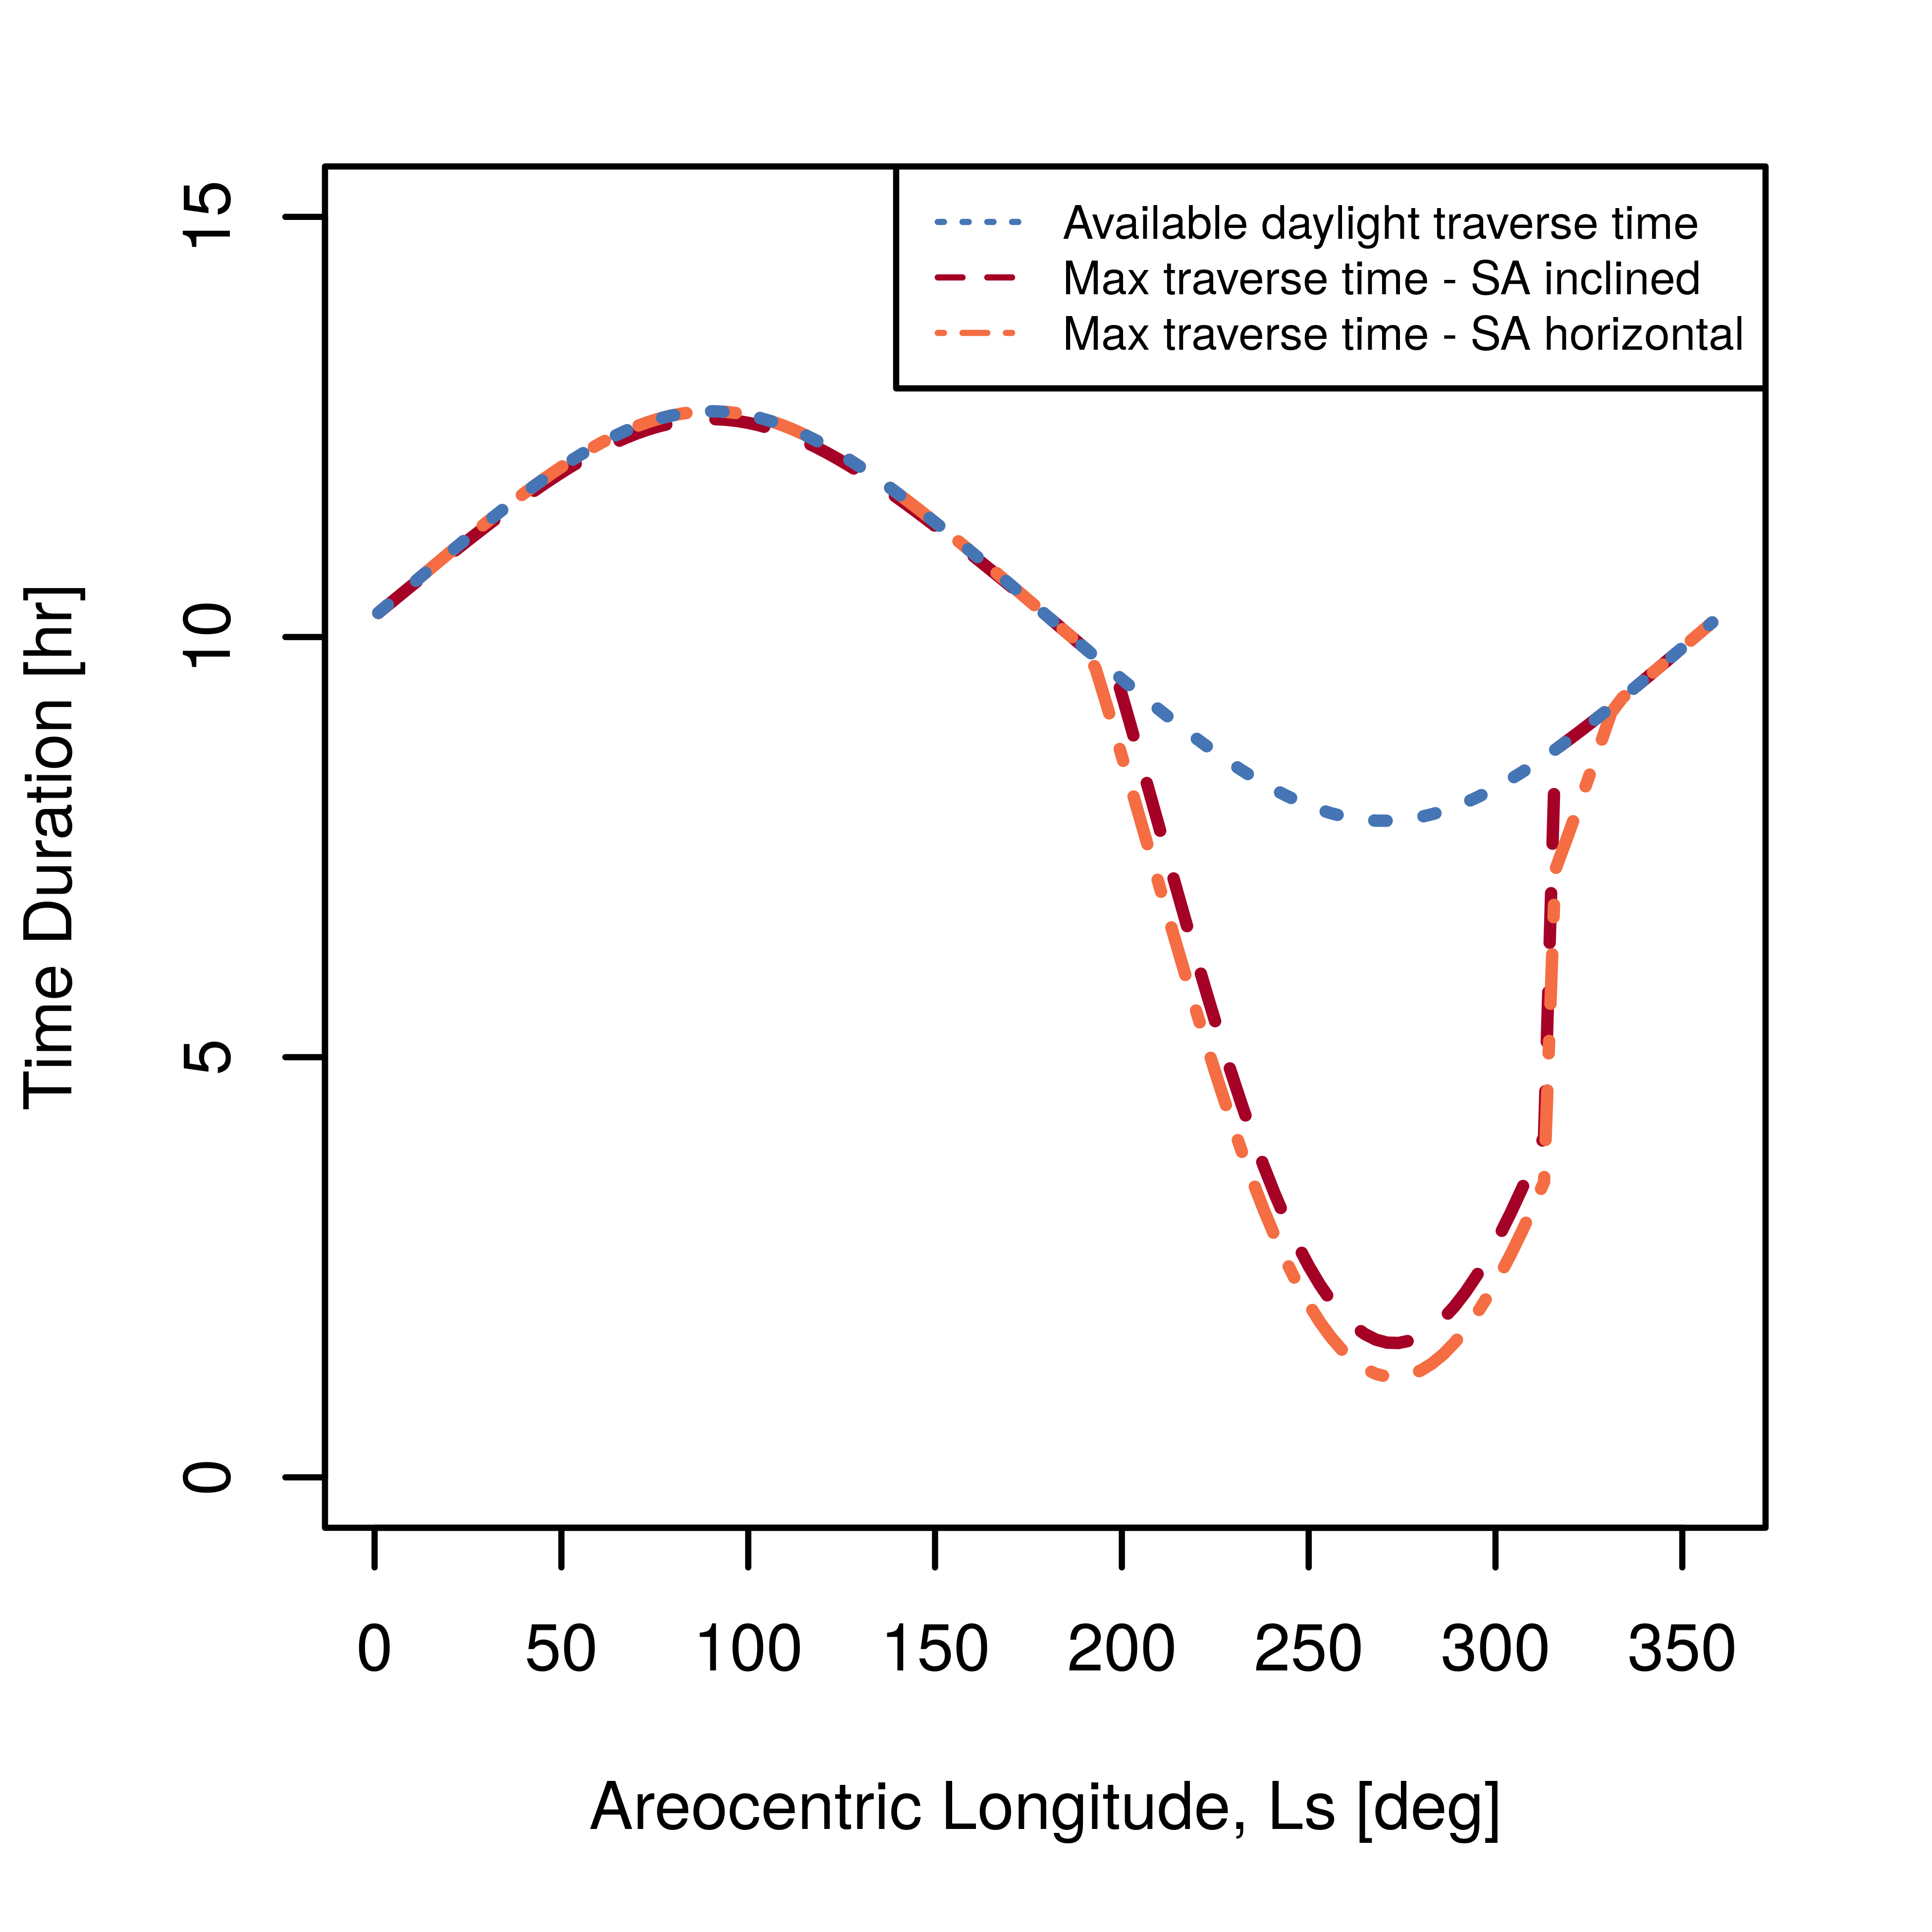
\includegraphics[height=\graphicsHeight]{figures/plots/ismeniuscavus-75w-max-traverse-durations-for-solar-cell-coverage-area-41m2.png}
    \subcaption{Maximum Traverse Durations}
    \label{fig:plot:sub:ismenius-cavus-max-traverse-durations}
  \end{subfigure}\\[0.8ex]
  \caption{Generated energy and maximum flat terrain traverse duration at Ismenius Cavus with solar cell coverage area of \SI{4.1}{m^{2}}. Surface inclination angle $\beta$ is \SI{10}{\degree}. $\tau$ factor 1 is used for global dust storm season ($\SI{185}{\degree} \leq L_{s} \leq \SI{315}{\degree}$) and 0.4 otherwise. The \textit{available daylight traverse time} corresponds to the amount of daylight hours left in a \textit{Traverse Sol} after subtracting the time taken by rover modes unrelated to traversing.}
  \label{fig:plot:ismenius-cavus-generated-energy-and-max-traverse-durations}
\end{figure}

However, no such ceiling can be observed for Iani Chaos in \refFig{fig:plot:iani-chaos-generated-energy-and-max-traverse-durations} which would explain the poor gains for that mission site scenario. In both cases, lack of traverse distance gains is more closely tied to the $\tau$ factor selected when defining the worst case reference Sol that drives \ac{SA} sizing. At high optical opacities, increased light scattering by airborne Martian dust results in $H_{\beta} \approx H_{h}$ due to diffuse insolation being the largest component in the global insolation. Thus, when \ac{SA} sizing for power generation during dusty Sols, the resulting inclined \ac{SA} surface yield little to no benefits over horizontal surfaces with respect to traverse distance gains as well as \ac{SA} mass and area.

\begin{figure}[h]
\captionsetup[subfigure]{justification=centering}
  \centering
  \setlength{\subfigureWidth}{0.24\textwidth}
  \setlength{\graphicsHeight}{40mm}
  \begin{subfigure}[t]{\subfigureWidth}
    \centering
    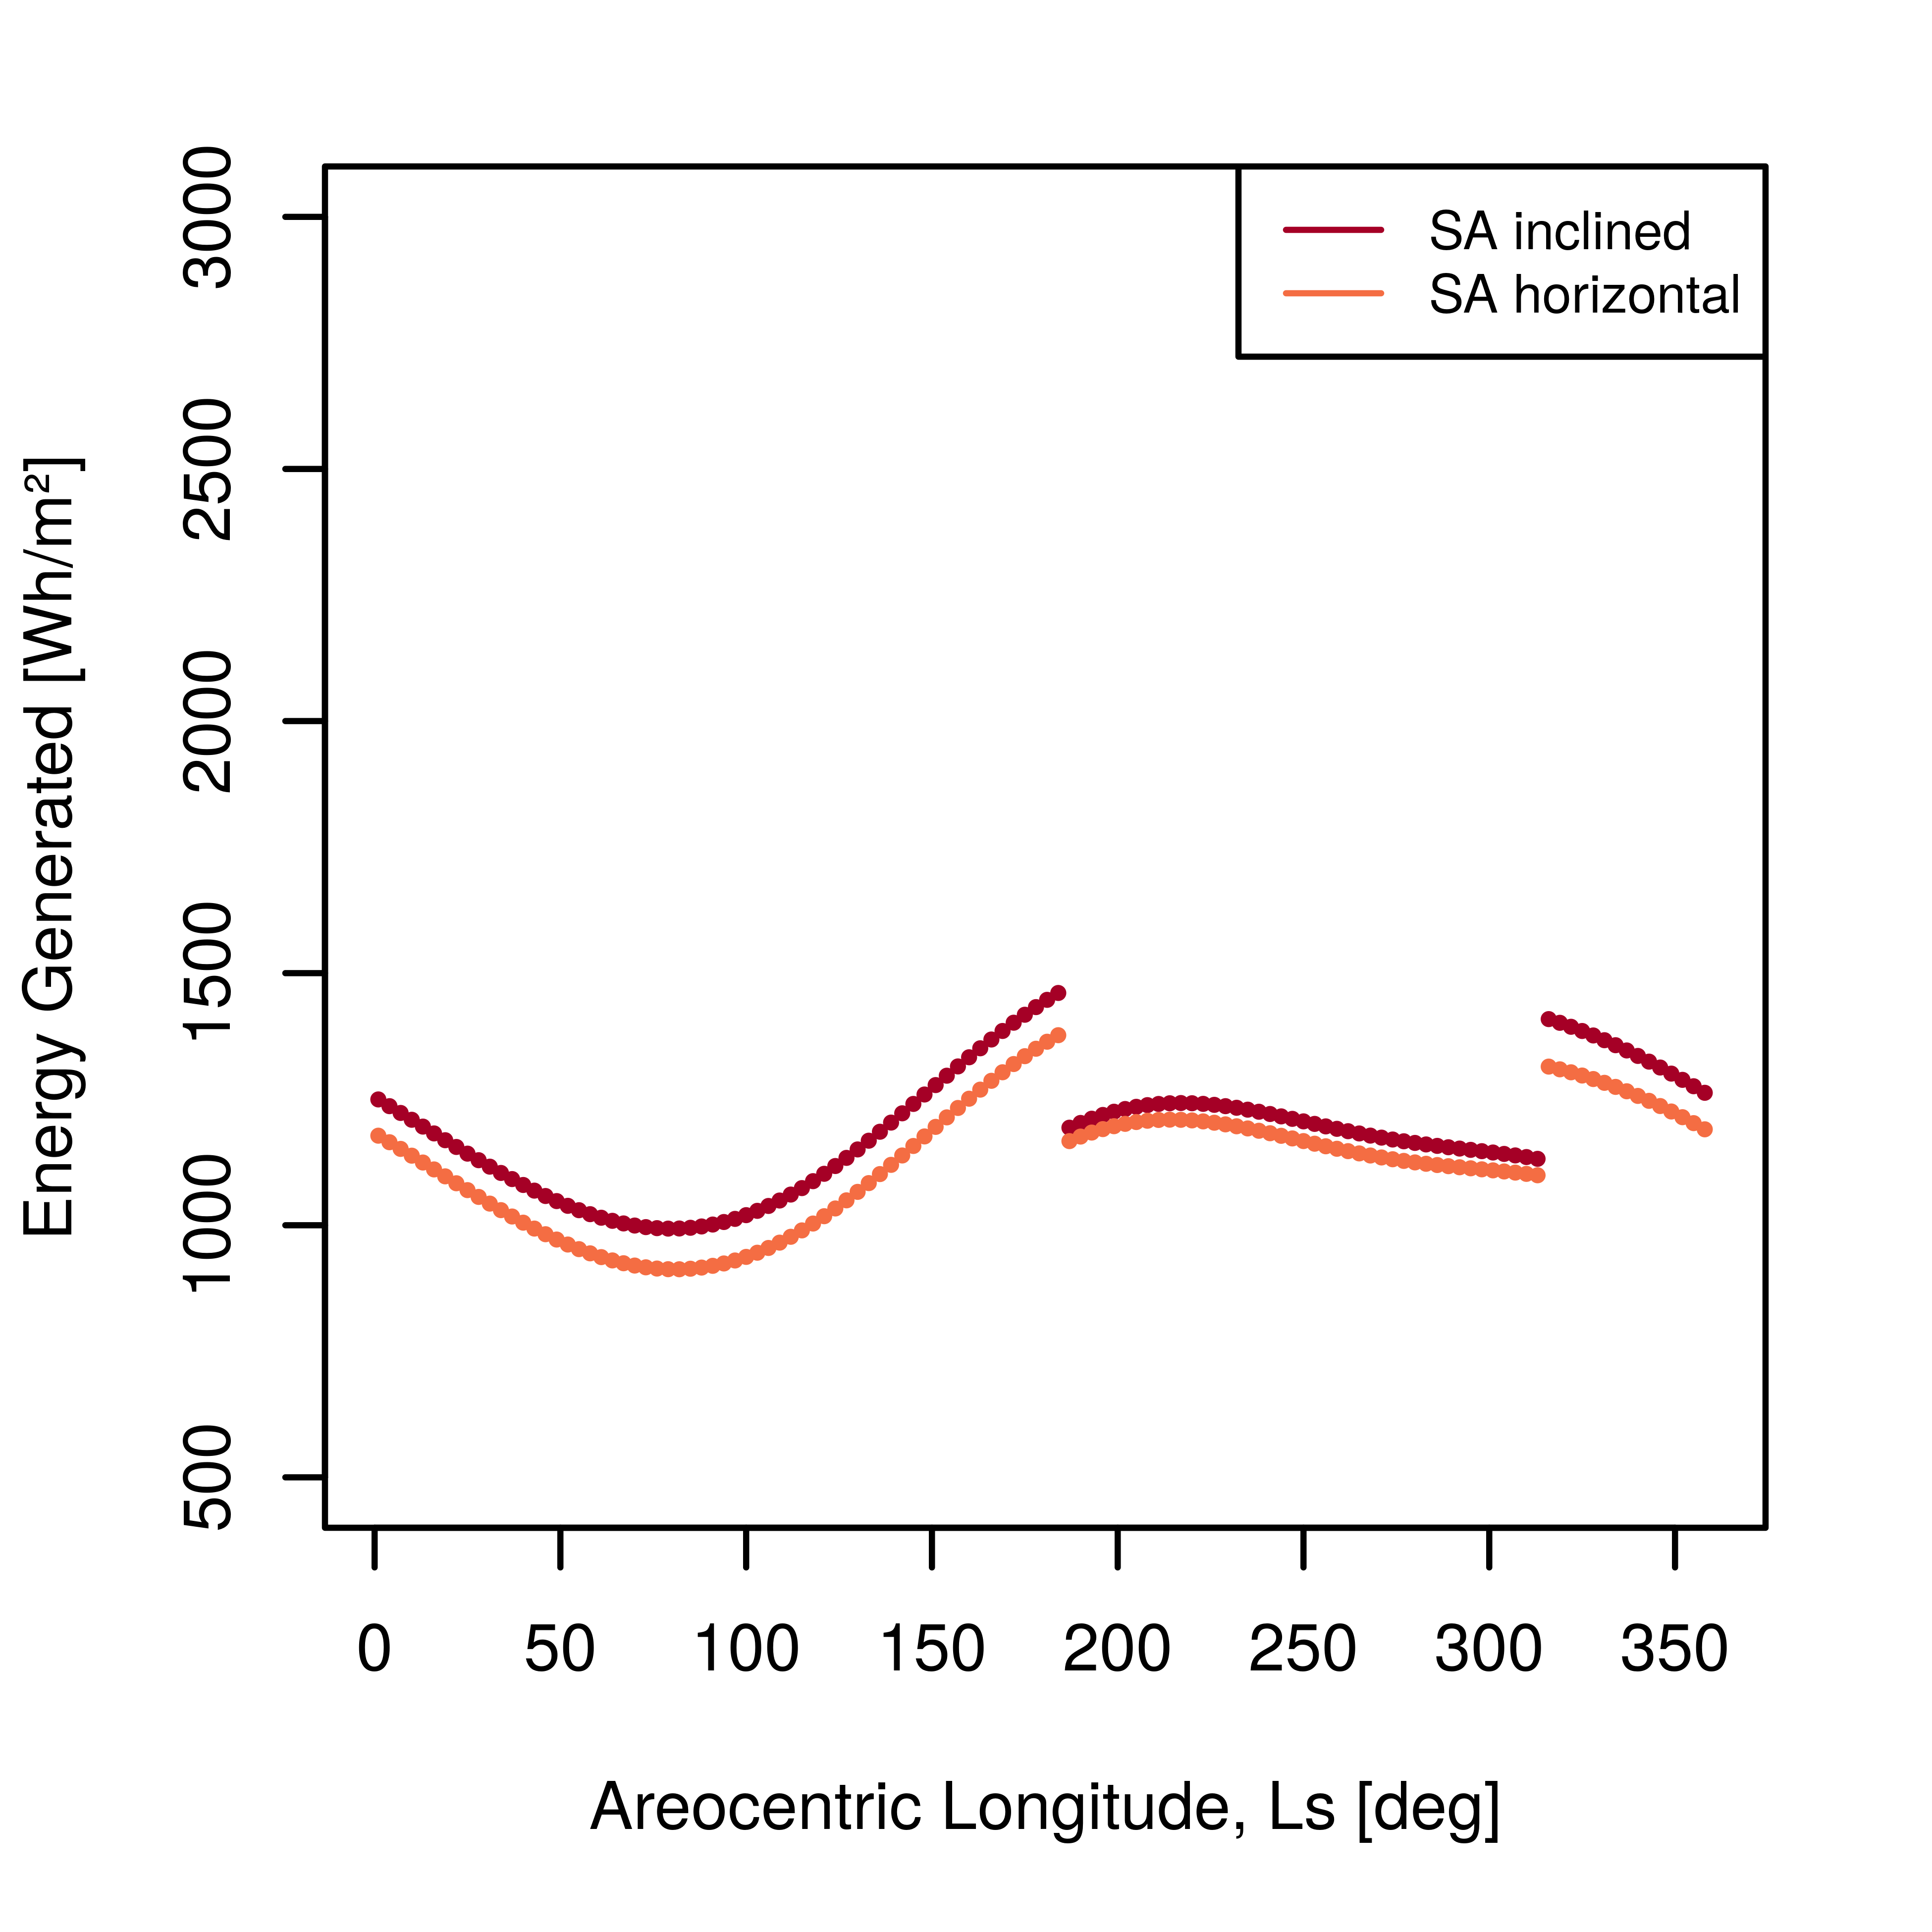
\includegraphics[height=\graphicsHeight]{figures/plots/ianichaos-daily-generated-energy-for-solar-cell-coverage-area-23m2.png}
    \subcaption{Generated Energy}
    \label{fig:plot:sub:iani-chaos-generated-energy}
  \end{subfigure}\hfill
  \begin{subfigure}[t]{\subfigureWidth}
    \centering
    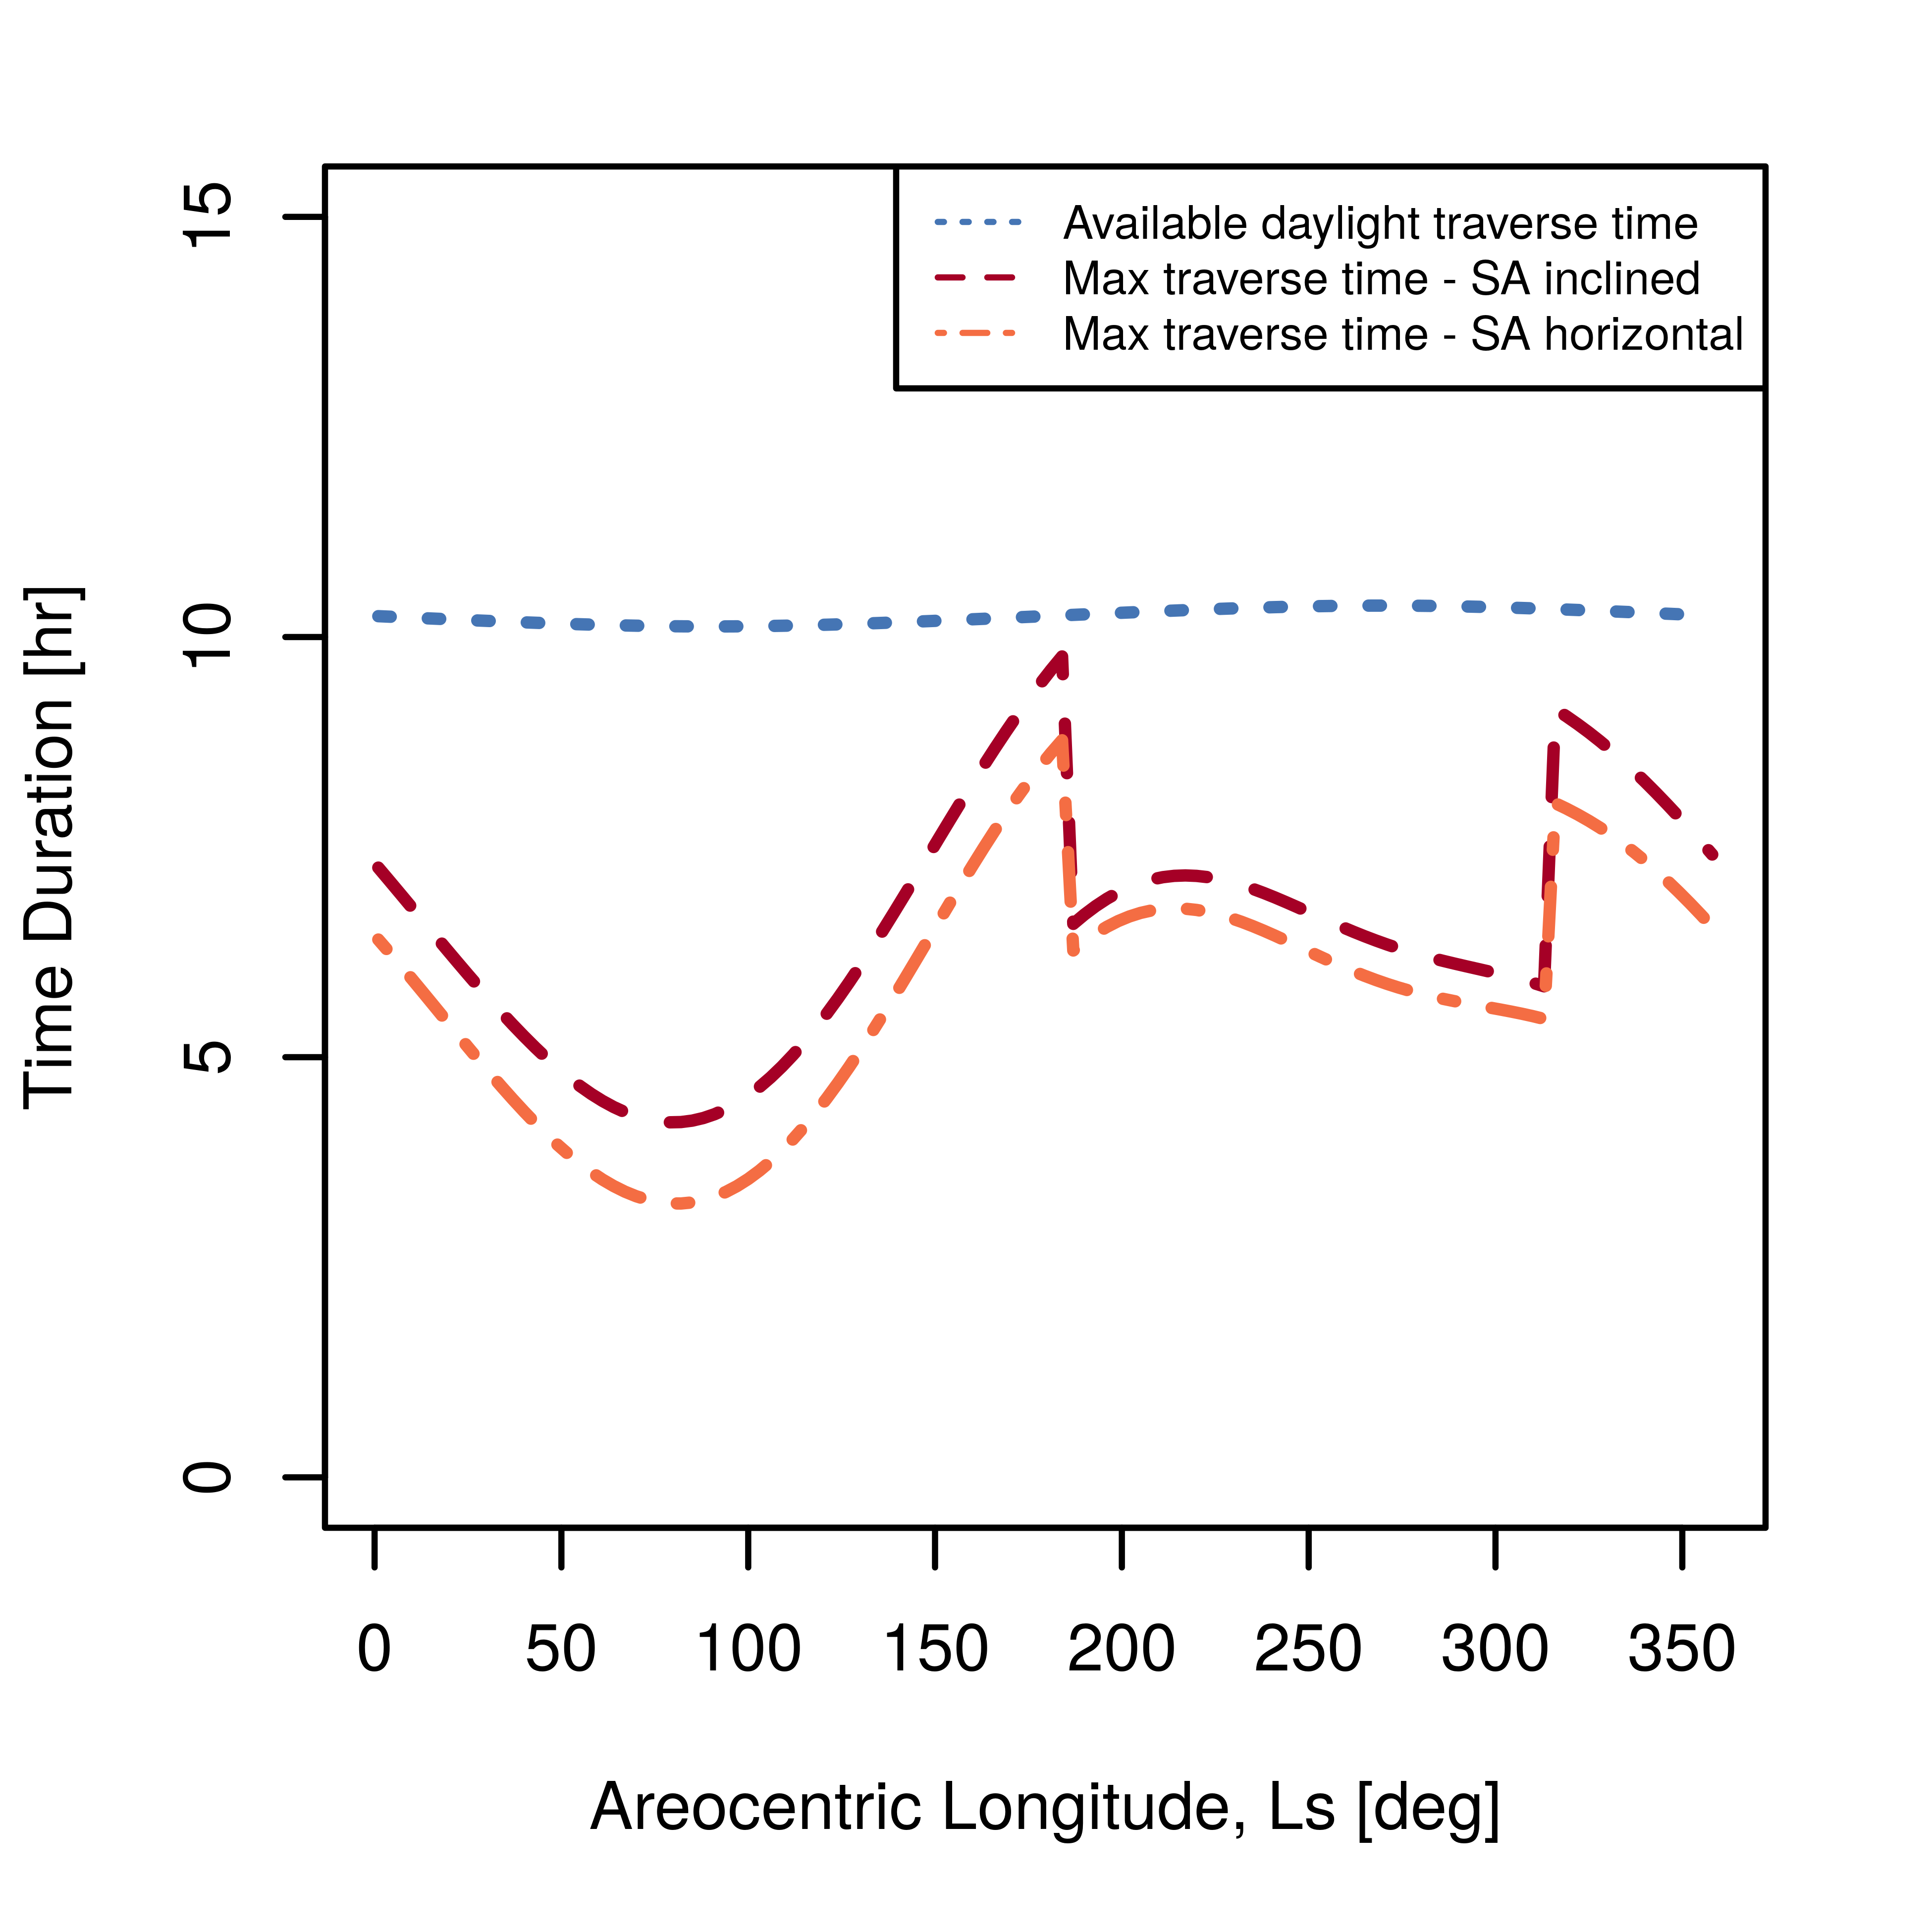
\includegraphics[height=\graphicsHeight]{figures/plots/ianichaos-75w-max-traverse-durations-for-solar-cell-coverage-area-23m2.png}
    \subcaption{Maximum Traverse Durations}
    \label{fig:plot:sub:iani-chaos-max-traverse-durations}
  \end{subfigure}\\[0.8ex]
  \caption{Generated energy and maximum flat terrain traverse duration at Iani Chaos with solar cell coverage area of \SI{2.3}{m^{2}}. The same considerations were taken as in \refFig{fig:plot:ismenius-cavus-generated-energy-and-max-traverse-durations}.}
  \label{fig:plot:iani-chaos-generated-energy-and-max-traverse-durations}
\end{figure}

The worst case power budget in \refTab{tab:worst-case-traverse-sol-power-budget} is set aside and the \ac{SA} sizing process is approached inversely by identifying solar cell coverage area targets based on the traverse distance gains brought about by an inclined surface. \refFig{fig:plot:flat-traverse-gains-for-different-sa-area} compares the traverse distance gains obtained with an inclined \ac{SA} surface for different solar cell coverage areas and optical depths.

\begin{figure}[h]
\captionsetup[subfigure]{justification=centering}
  \centering
  \setlength{\subfigureWidth}{0.24\textwidth}
  \setlength{\graphicsHeight}{40mm}
    \begin{subfigure}[t]{\subfigureWidth}
      \centering
      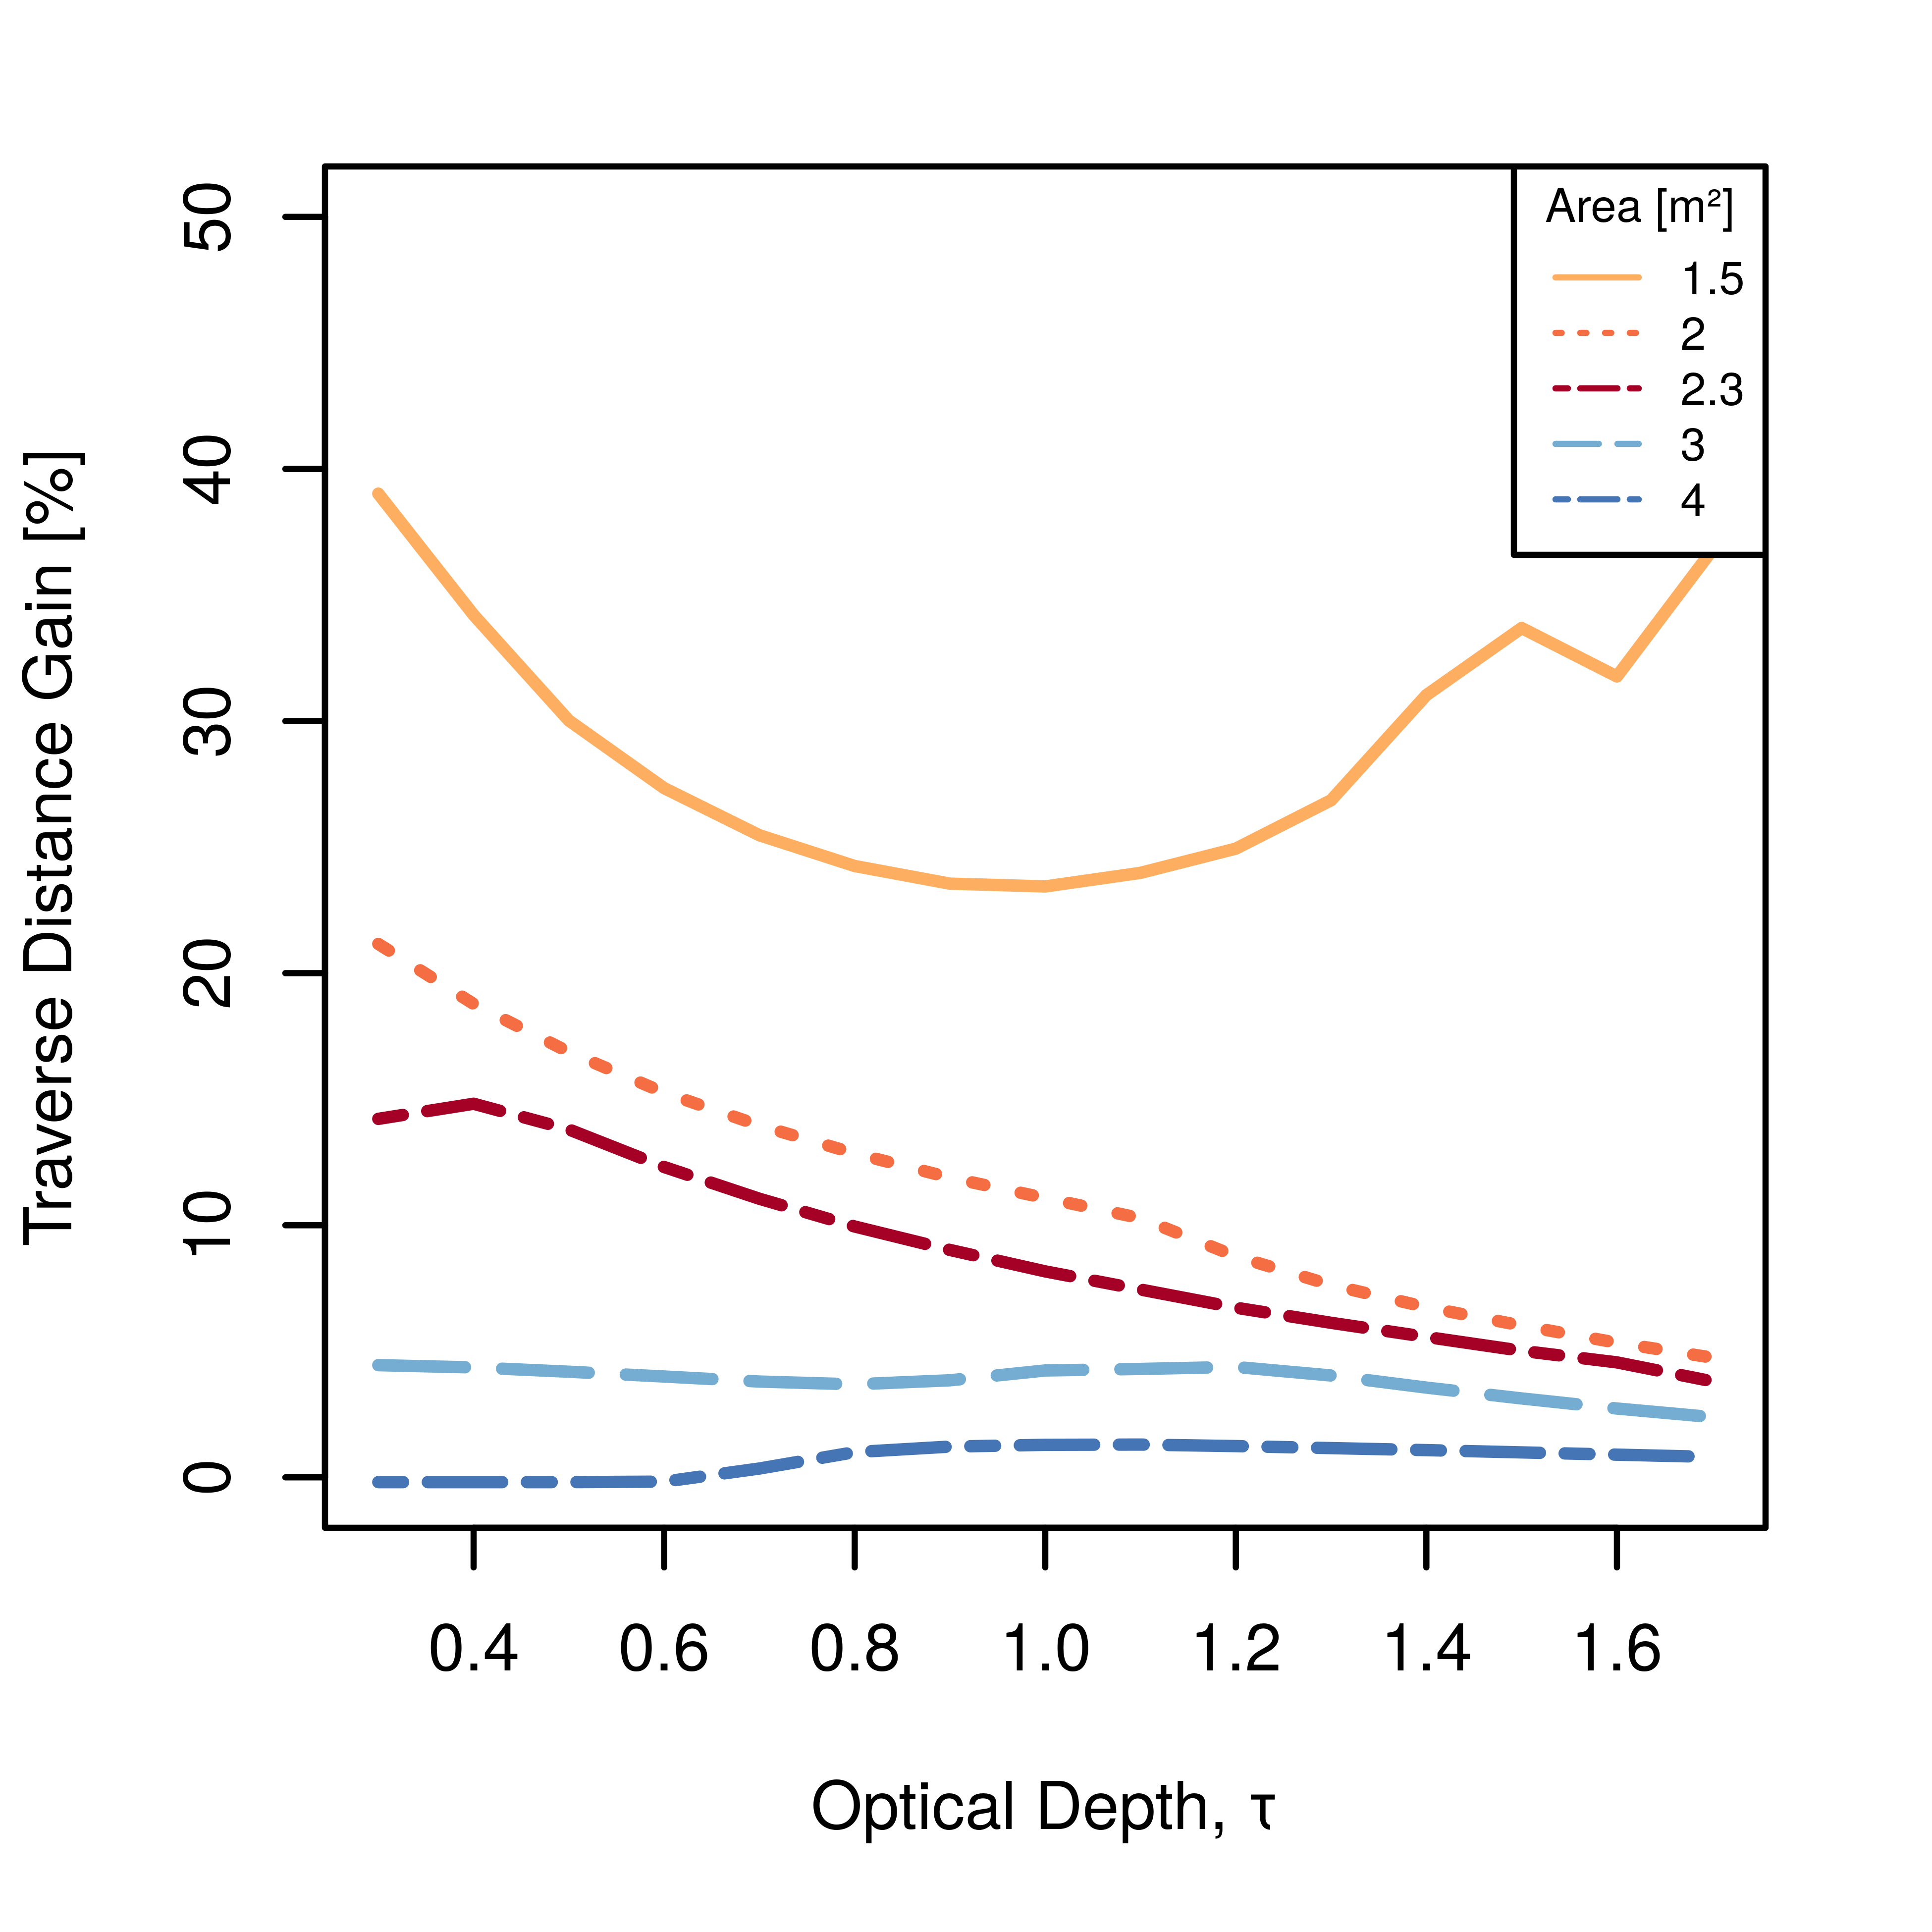
\includegraphics[height=\graphicsHeight]{figures/plots/ianichaos-75w-traverse-gains-for-different-solar-cell-coverage-areas.png}
    \subcaption{Iani Chaos}
    \label{fig:plot:sub:ismenius-chaos-flat-traverse-gains-for-different-sa-area}
    \end{subfigure}\hfill
    \begin{subfigure}[t]{\subfigureWidth}
      \centering
      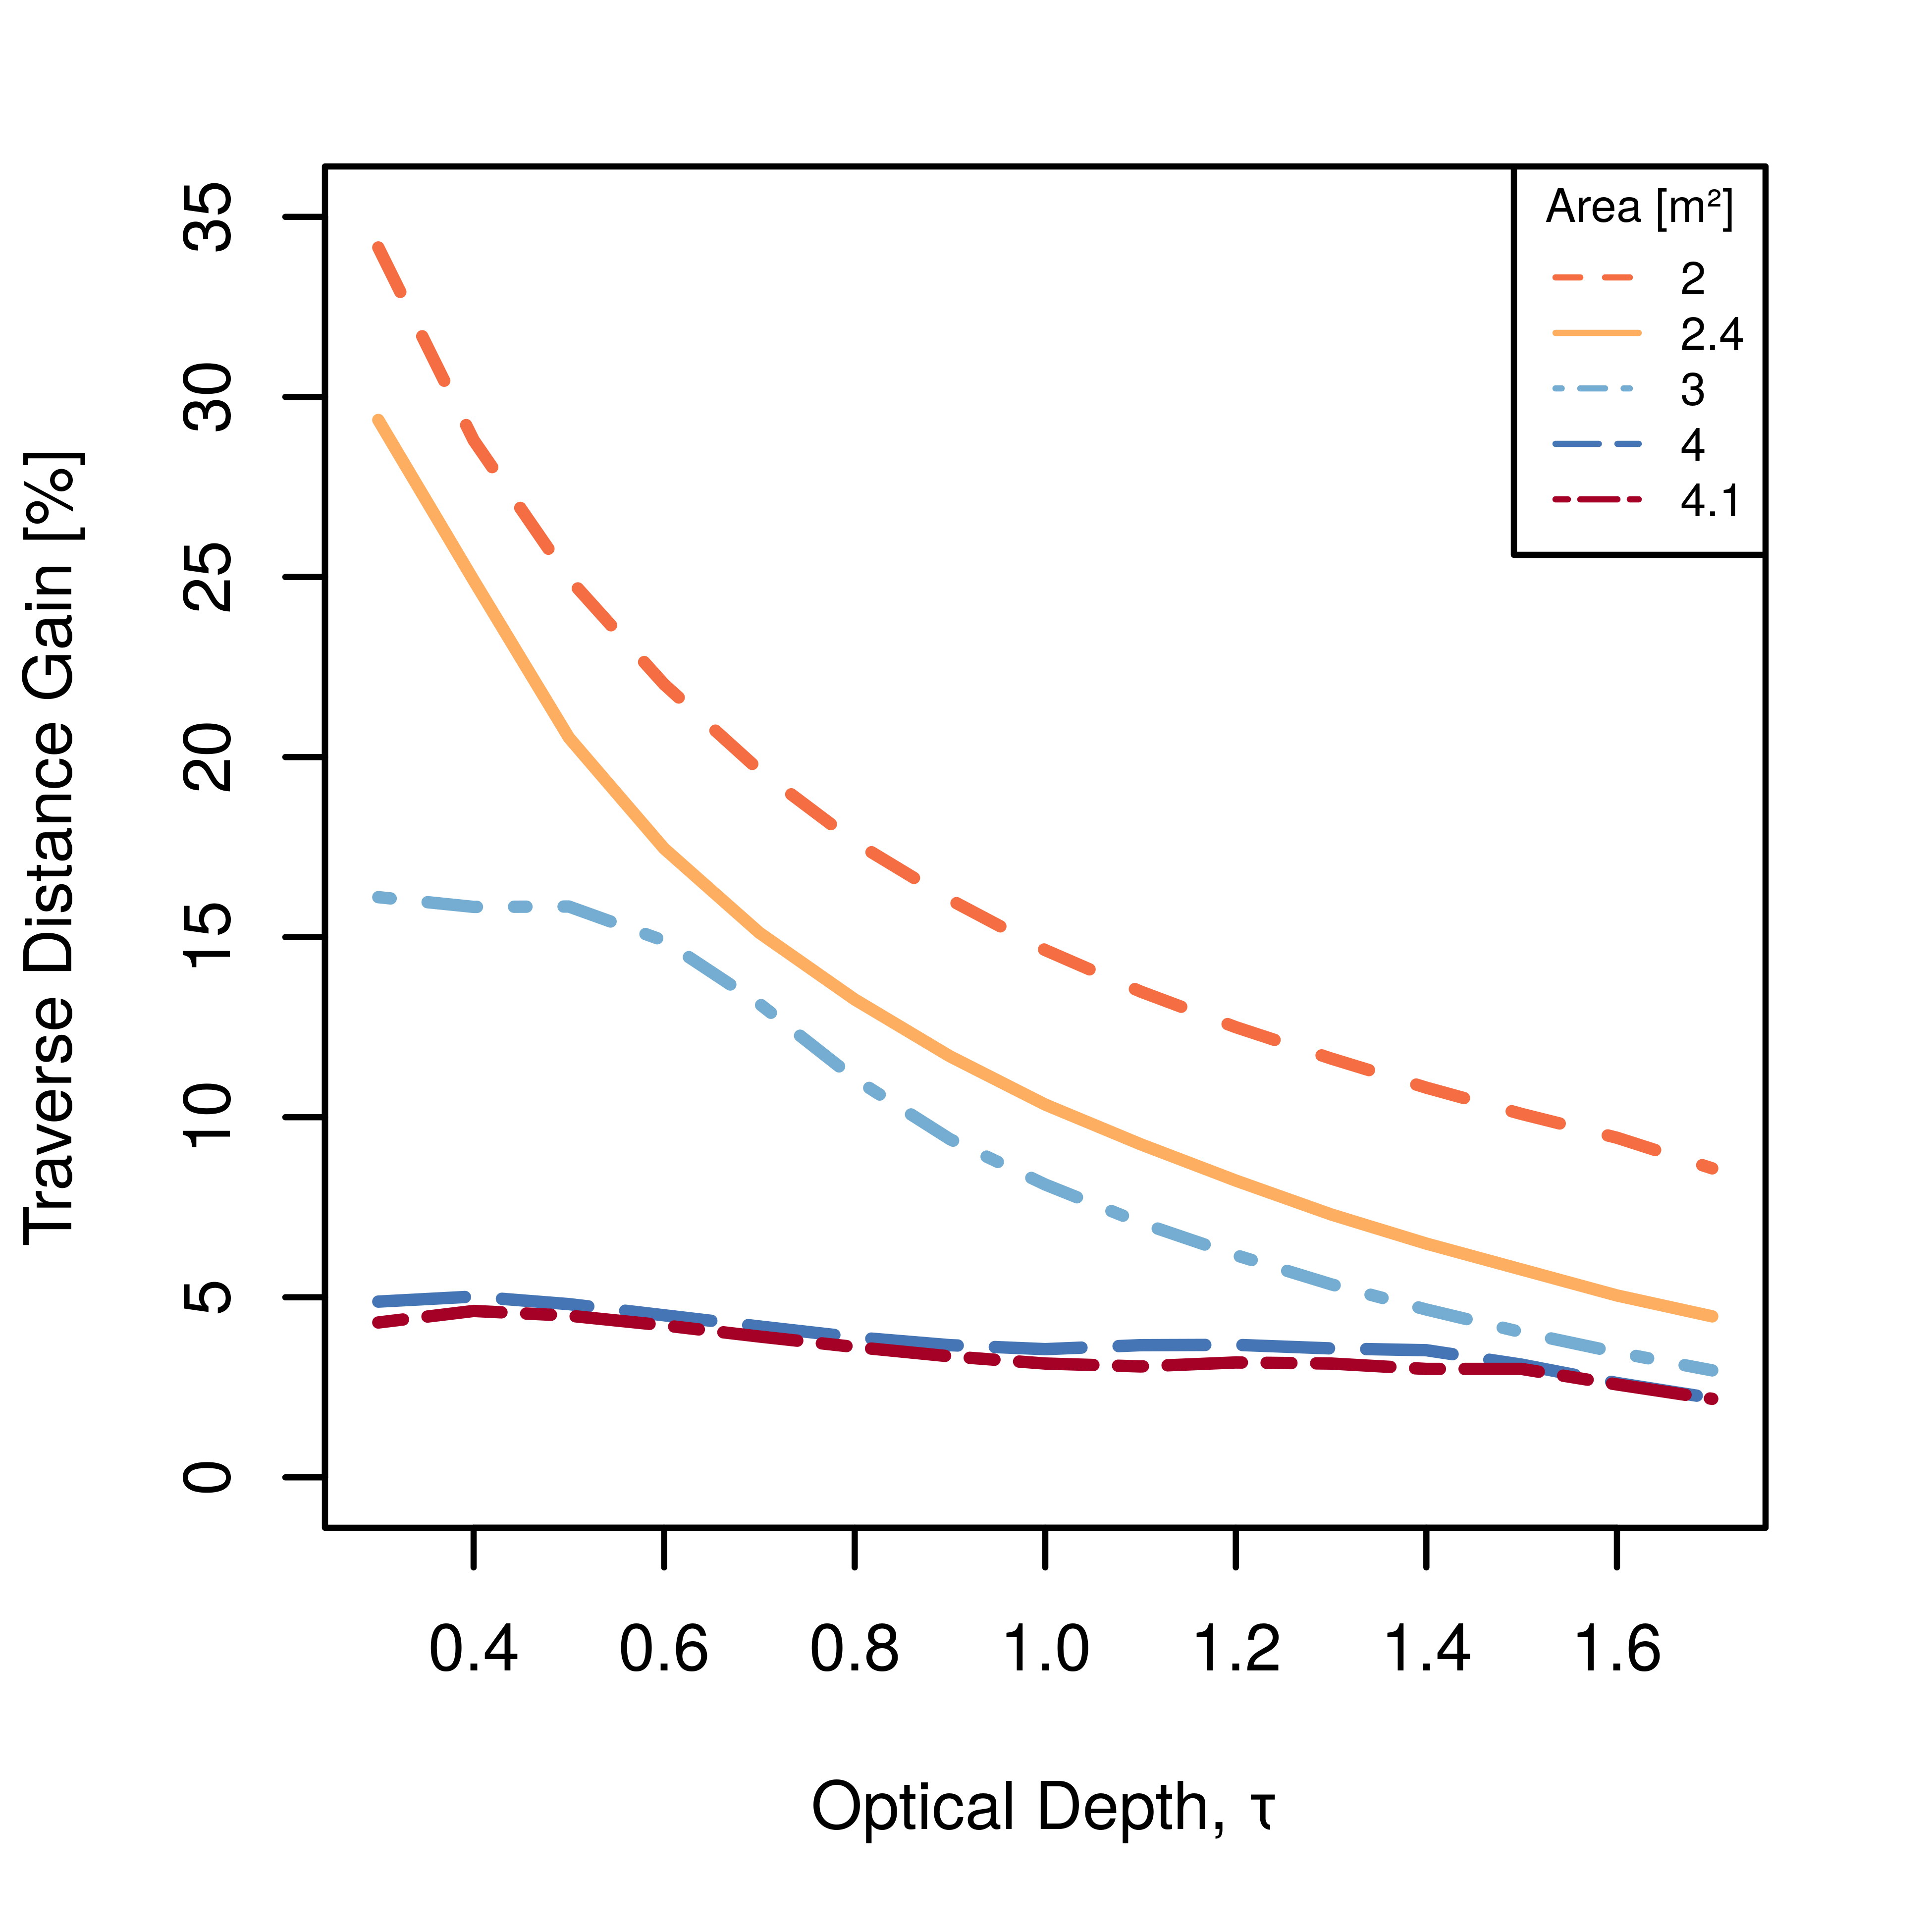
\includegraphics[height=\graphicsHeight]{figures/plots/ismeniuscavus-75w-traverse-gains-for-different-solar-cell-coverage-areas.png}
    \subcaption{Ismenius Cavus}
    \label{fig:plot:sub:iani-chaos-flat-traverse-gains-for-different-sa-area}
    \end{subfigure}\\[0.8ex]
    \caption{Average flat terrain traverse distance gains at mission sites for different solar cell coverage areas. \ac{SA} inclination angle $\beta_{max} = \SI{10}{\degree}$ with orientation angles $\gamma_{c}$ set to their optimal values for the considered traverse Sols.}
    \label{fig:plot:flat-traverse-gains-for-different-sa-area}
\end{figure}

Targeting a solar cell coverage area of \SI{1.5}{m^{2}} at Iani Chaos results in an average \SI{34}{\percent} gain in traverse for a clear day at $\tau$ factor 0.4. The gain remains significant at \SI{23}{\percent} for a dusty day at $\tau$ factor 1. The increase in gain observe for $\tau$ factors greater than 1 are inconsequentially tied to negligible distances. At Ismenius cavus, a solar cell coverage area of \SI{2.4}{m^{2}} results in \SI{25}{\percent} and \SI{10}{\percent} gains for $\tau$ factor 0.4 and 1, respectively. Applying the same packing efficiency and \ac{SA} surface density as the initial sizing results in \ac{SA} areas of \SI{1.7}{m^{2}} at Iani Chaos with a mass of \SI{6.3}{\kilo\gram} and \SI{2.8}{m^{2}} at Ismenius Cavus with a mass of \SI{10.4}{\kilo\gram}. The maximum daily traverse durations attainable at both sites with these target \ac{SA} areas are shown in \refFig{fig:plot:final-maximum-traverse-durations-at-missions-sites}. However, these gains come with significantly reduced maximum flat traverse distance coverage of \SI{12}{\kilo\meter} at Iani Chaos and \SI{35}{\kilo\meter} at Ismenius Cavus. Mission design with or without \ac{SA} surface inclination thus not only depend on \ac{SA} size and mass constraints but also on mission requirements with respect to target traverse coverages.


\begin{figure}[h]
\captionsetup[subfigure]{justification=centering}
  \centering
  \setlength{\subfigureWidth}{0.24\textwidth}
  \setlength{\graphicsHeight}{40mm}
  \begin{subfigure}[t]{\subfigureWidth}
    \centering
    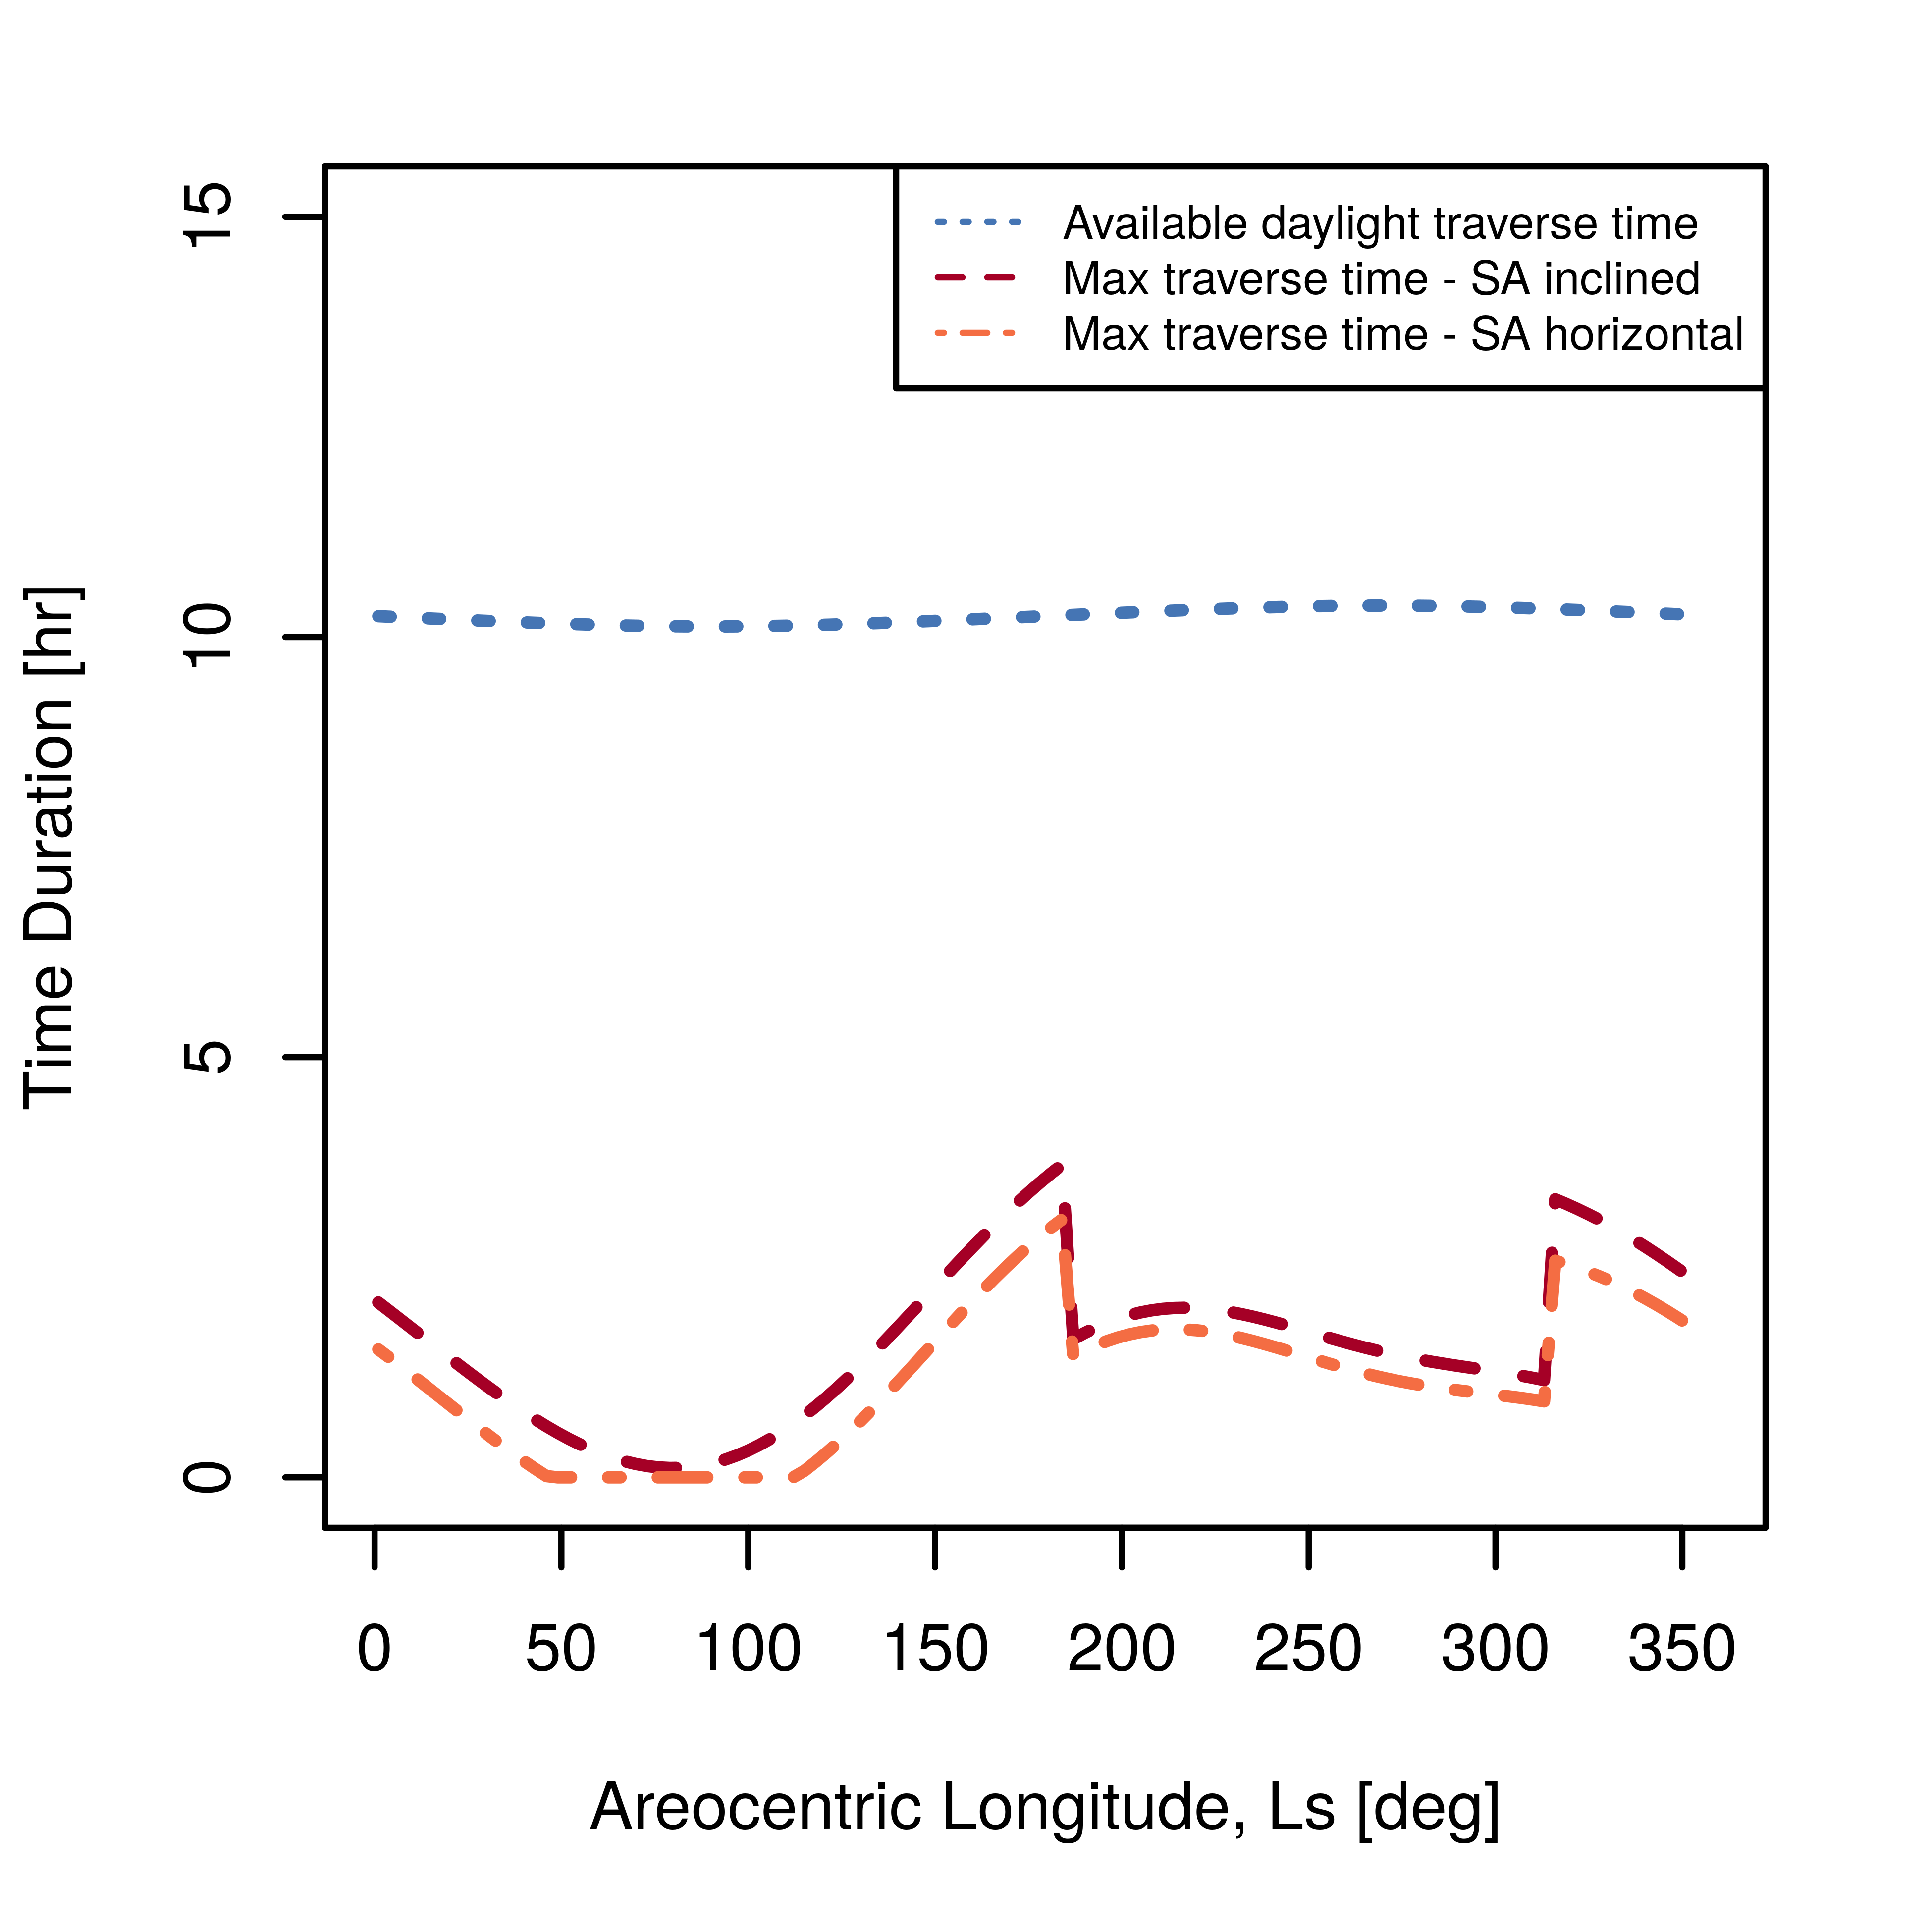
\includegraphics[height=\graphicsHeight]{figures/plots/ianichaos-75w-max-traverse-durations-for-solar-cell-coverage-area-15m2.png}
    \subcaption{Iani Chaos, solar cell coverage = \SI{1.5}{m^{2}}}
    \label{fig:plot:sub:final-maximum-traverse-durations-iani-chaos}
  \end{subfigure}\hfill
  \begin{subfigure}[t]{\subfigureWidth}
    \centering
    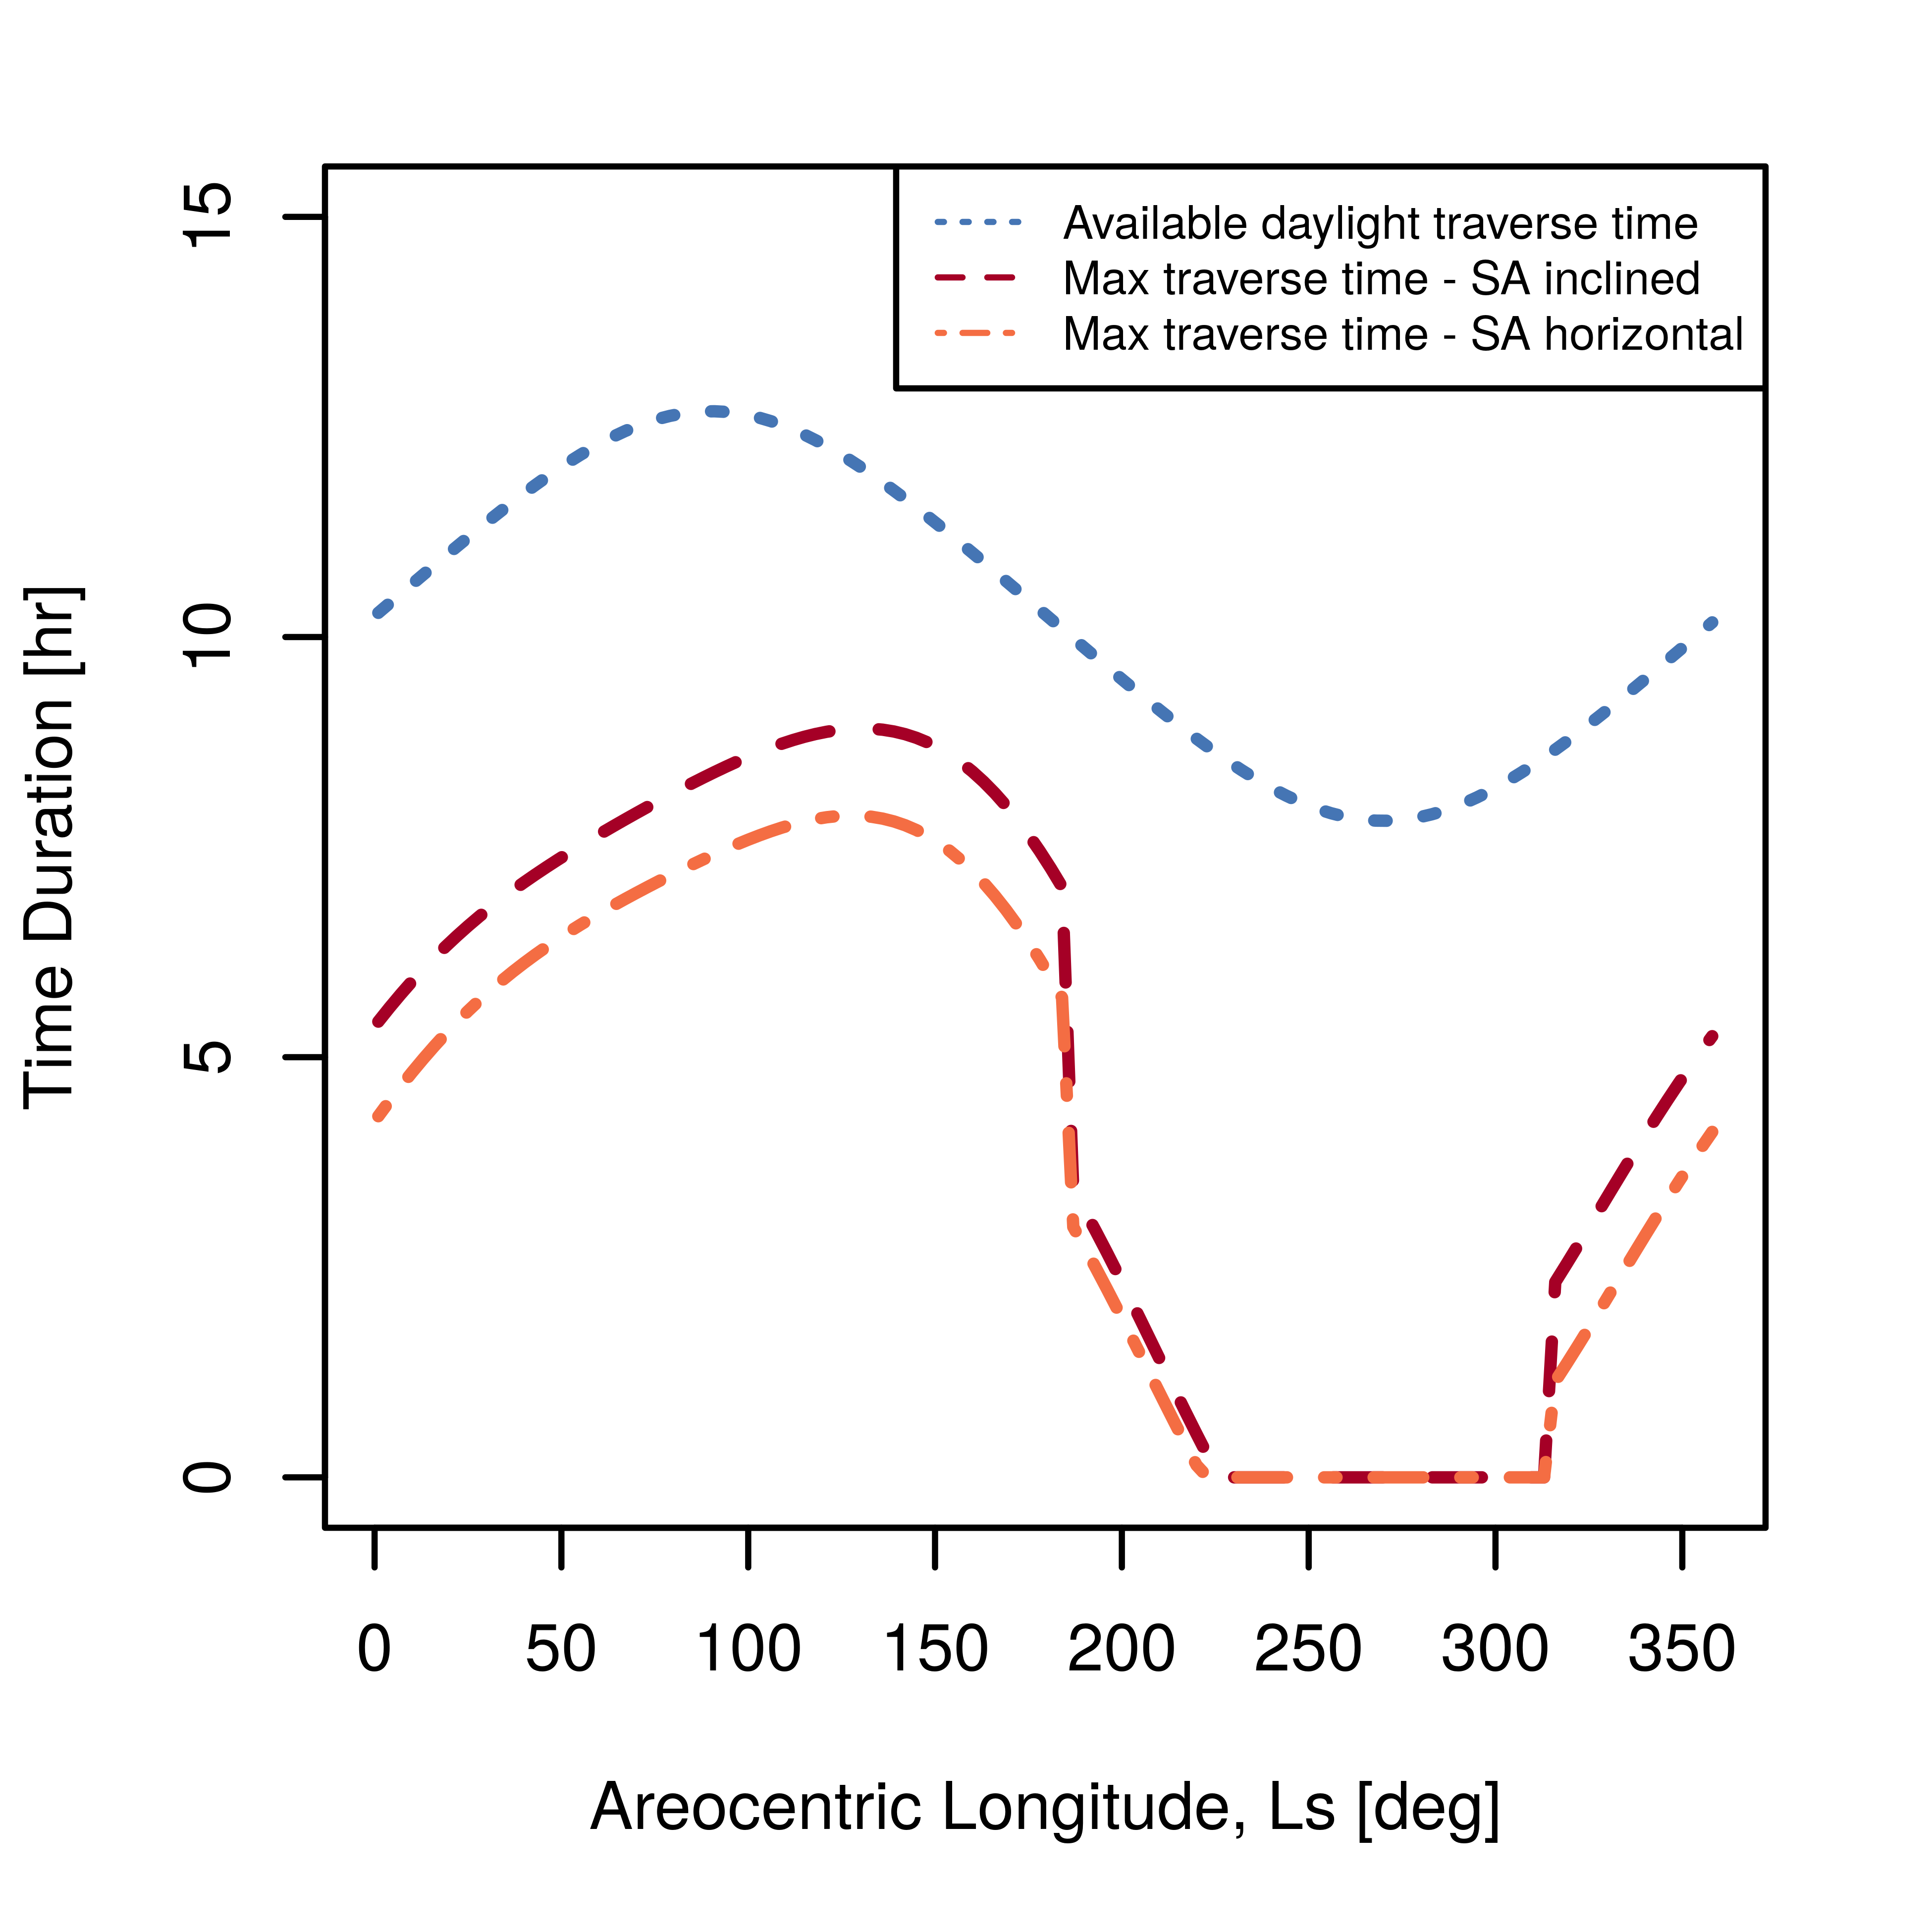
\includegraphics[height=\graphicsHeight]{figures/plots/ismeniuscavus-75w-max-traverse-durations-for-solar-cell-coverage-area-24m2.png}
    \subcaption{Ismenius Cavus, solar cell coverage area = \SI{2.4}{m^{2}}}
    \label{fig:plot:sub:final-maximum-traverse-durations-ismenius-cavus}
  \end{subfigure}\\[0.8ex]
  \caption{Maximum traverse durations at mission sites. The same considerations were taken as in \refFig{fig:plot:ismenius-cavus-generated-energy-and-max-traverse-durations}.}
  \label{fig:plot:final-maximum-traverse-durations-at-missions-sites}
\end{figure}

\ac{SA} sizing with the hibernation reference Sol power budget defined in \refTab{tab:hibernation-sol-power-budget} as the worst case power budget fails to meet the target \ac{SA} areas. However, the required power draws only differ by a few Watts. At Iani Chaos, this is achieved by reducing the hibernation mode power draws from \SI{18}{\watt} to \SI{17}{\watt}. At Ismenius Cavus, hibernation power draws need to be reduced from \SI{18}{\watt} to \SI{15}{\watt}. Taking into account a \SI{20}{\percent} system margin, the energy requirement for hibernation Sols become \SI{490}{\watt\hour} at Iani Chaos for a \SI{1.7}{m^{2}} \ac{SA} area and \SI{432}{\watt\hour} at Ismenius Cavus for a \SI{2.8}{m^{2}} \ac{SA} area. A first iteration of the rover with a \ac{SA} for an Ismenius Cavus deployment is shown in \refFig{fig:solar-array-on-ismenius-cavus-chaos}.


\begin{figure}[h]
 \centering
 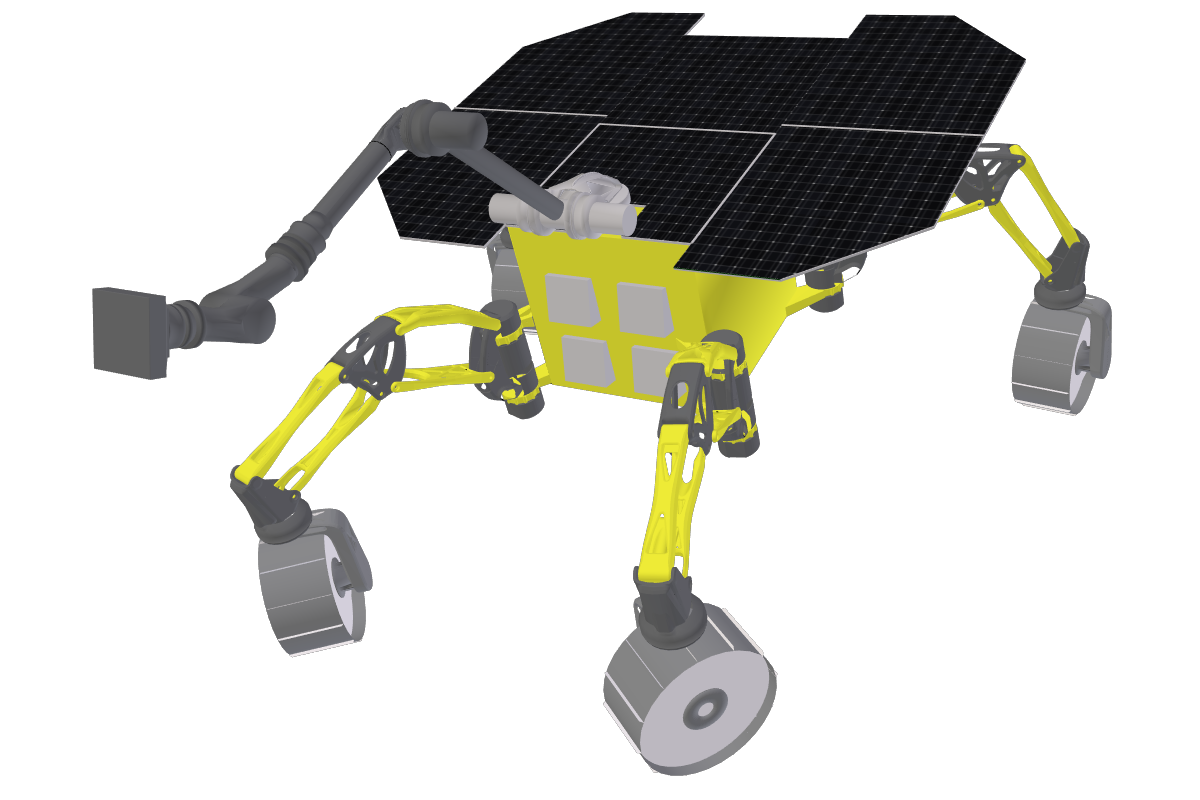
\includegraphics[width=3.25in]{figures/images/ismenius-cavus-10deg-pitch.png}\\
 \caption{Rover with \ac{SA} for Ismenius Cavus deployment.}
 \label{fig:solar-array-on-ismenius-cavus-chaos}
\end{figure}



%%%%%%%%%%%%%%%%%%%%%%%%%%%%%%%%%%%%%%%%%%%
\section{Simulation}
%%%%%%%%%%%%%%%%%%%%%%%%%%%%%%%%%%%%%%%%%%%
The proposed rover and \ac{SA} configurations are modeled with Blender/Phobos and loaded into MARS for mission scenario simulation. Phobos is ``an add-on for the open-source 3D modeling software Blender that enables the creation of robot models for use in robot frameworks like ROS and ROCK or in real-time simulations such as MARS'' \cite{Phobos}. MARS is ``a cross-platform simulation and visualization tool created for robotics research. It consists of a core framework containing all main simulation components, a GUI (based on Qt), 3D visualization (using OSG) and a physics engine (based on ODE)'' \cite{MARSSim}.

\subsection{Z-Axis Revolutions}

\refFig{fig:sub:simulation-data-rover-revolution-generated-power-line-chart} and \refFig{fig:sub:simulation-data-rover-revolution-generated-power-polar-chart} are two different representations of the same solar power output obtained from commanding the rover to execute a \SI{10}{\degree} forward body-pitch followed by several revolutions around its z-axis. These revolutions result in a sinusoidal power output variation. Local spikes and dips are noted around \SI{100}{\second} and \SI{160}{\second} due to small changes in the \ac{SA} inclination and orientation angles caused by the rover driving over uneven terrain. In \refFig{fig:sub:simulation-data-rover-revolution-generated-power-polar-chart}, the angle values represent the direction faced by the inclined \ac{SA}. Maximum power is generated when the \ac{SA} is oriented southwards, towards the equator, in the general direction of the sun. Inversely, facing northwards, away from the sun, generates the least amount of power.

\begin{figure}[h]
  \captionsetup[subfigure]{justification=centering}
  \centering
  \setlength{\subfigureWidth}{0.24\textwidth}
  \setlength{\graphicsHeight}{40mm}
  \begin{subfigure}[t]{\subfigureWidth}
    \centering
    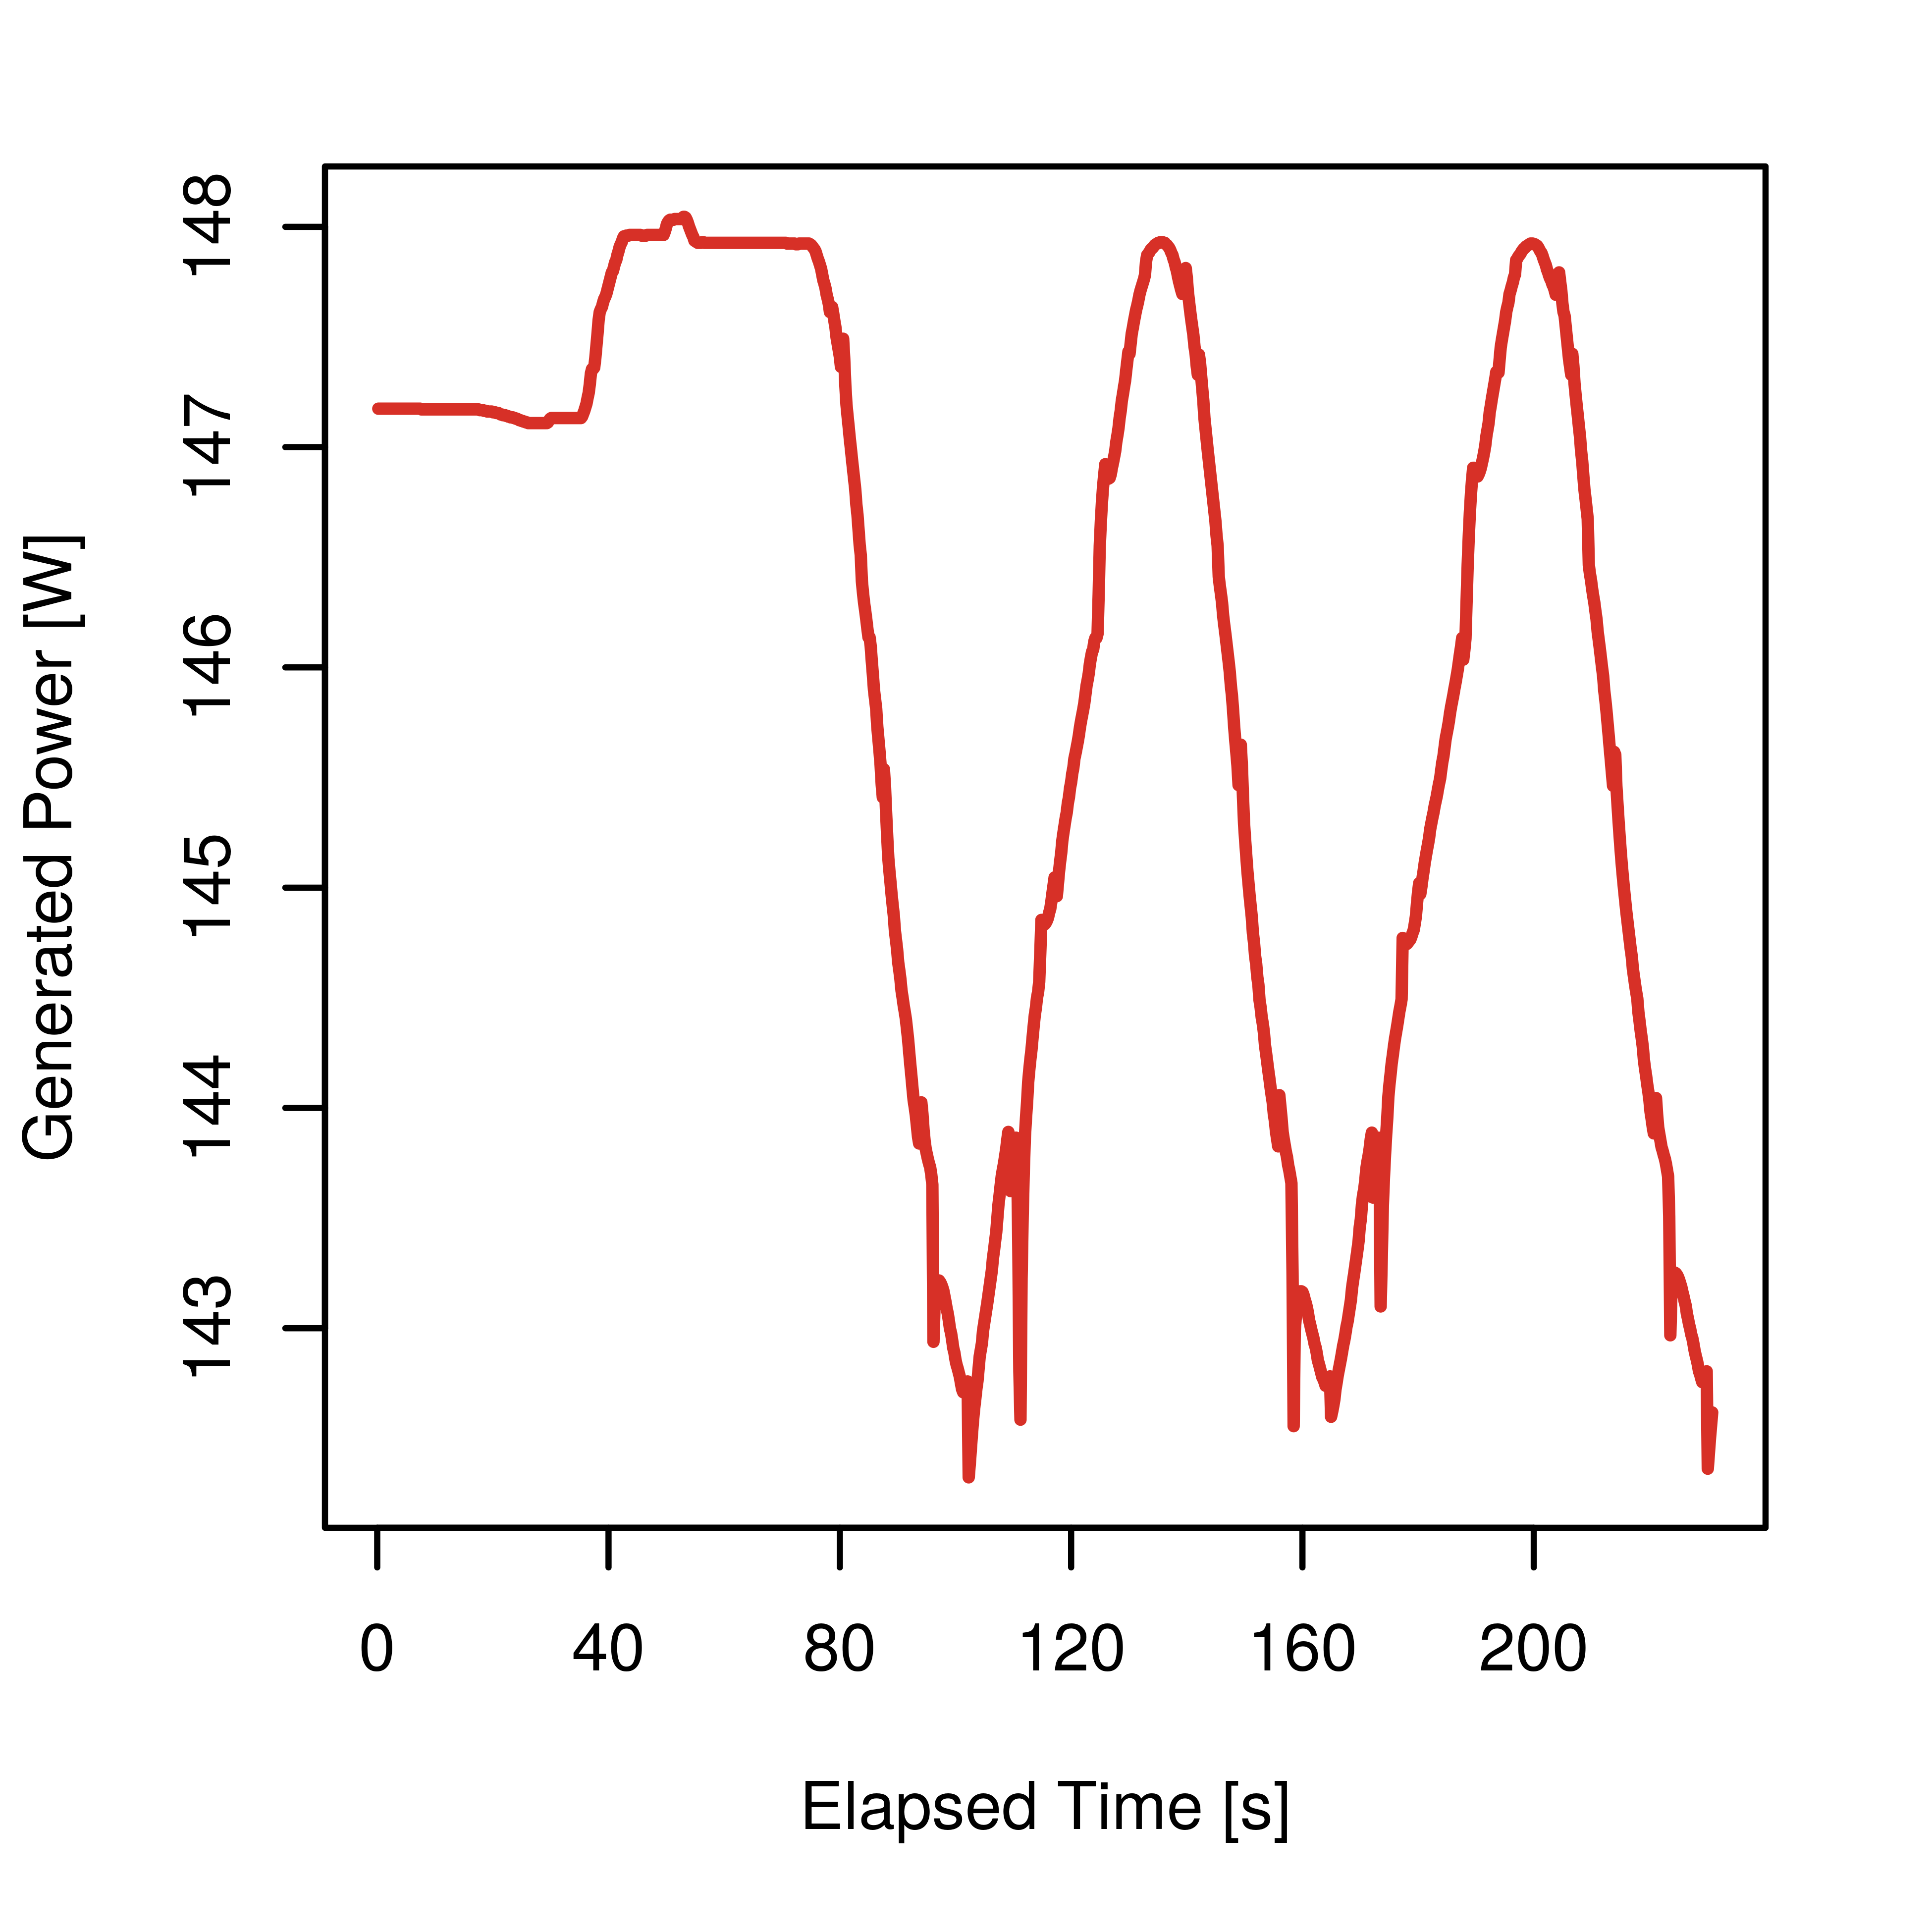
\includegraphics[height=\graphicsHeight]{figures/plots/zaxis-revolutions.png}
    \subcaption{Line chart}
    \label{fig:sub:simulation-data-rover-revolution-generated-power-line-chart}
  \end{subfigure}\hfill
  \begin{subfigure}[t]{\subfigureWidth}
    \centering
    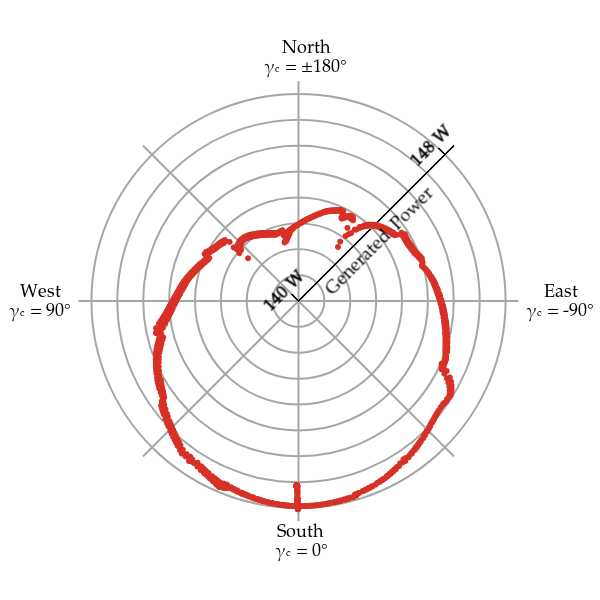
\includegraphics[height=\graphicsHeight]{figures/plots/zaxis-revolutions-polar.png}
    \subcaption{Polar chart}
    \label{fig:sub:simulation-data-rover-revolution-generated-power-polar-chart}
  \end{subfigure}\\[0.6ex]
  \caption{Power generated by the rover's \ac{SA} for multiple revolutions along its z-axis. Simulation condition is solar noon at Ismenius Cavus with $\beta \approx \SI{10}{\degree}$. In the polar chart, angle values represent the direction faced by the inclined \ac{SA} where \SI{0}{\degree} is South (towards the equator), \SI{-90}{\degree} is East, \SI{180}{\degree} is North, and \SI{90}{\degree} is West.}
  \label{fig:simulation-data-rover-revolution-generated-power}
\end{figure}

\subsection{Slope Compensation}

The worst case slope traverse is on an inclined surface facing away from the sun. The rover's active suspension system can be used to reduce the \ac{SA} inclination angle by commanding a rover body pitch in the opposite direction. This slope compensation scenario is illustrated in \refFig{fig:sub:rover-on-slope-beta} where $B$ denotes the slope surface inclination angle and $\beta$ the \ac{SA} surface inclination angle.

\begin{figure}[h]
\captionsetup[subfigure]{justification=centering}
  \centering
  \begin{subfigure}[t]{\subfigureWidth}
    \centering
    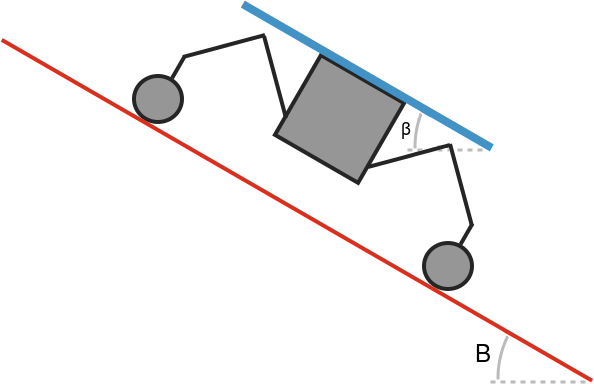
\includegraphics[height=\graphicsHeight]{figures/images/stick-rover-beta-large.png}
    \subcaption{$\beta = B$}
    \label{fig:sub:rover-on-slope-beta-large}
  \end{subfigure}\hfill
  \begin{subfigure}[t]{\subfigureWidth}
    \centering
    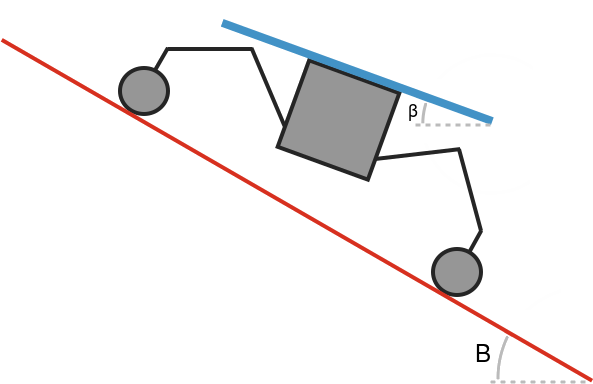
\includegraphics[height=\graphicsHeight]{figures/images/stick-rover-beta-small.png}
    \subcaption{$\beta < B$}
    \label{fig:sub:rover-on-slope-beta-small}
  \end{subfigure}\\[0.8ex]
  \caption{Slope compensation with active suspension system to reduce the \ac{SA} surface inclination angle. Slope inclination angle $B = \SI{30}{\degree}$. In (a), $\beta = B = \SI{30}{\degree}$. In (b), the rover is tilted \SI{10}{\degree} in the opposite direction of the slope so that $\beta = \SI{20}{\degree}$.}
  \label{fig:sub:rover-on-slope-beta}
\end{figure}

By way of example, at Ismenius Cavus for a $\tau$ factor of 0.4 and an areocentric longitude $L_{s}$ of \SI{270}{\degree}, descending a \SI{30}{\degree} slope bearing North results in a daily insolation of \SI{319}{Whm^{-2}}. This is increased to \SI{767}{Whm^{-2}} by decreasing $\beta$ from \SI{30}{\degree} to \SI{25}{\degree} after tilting the rover southwards by \SI{5}{\degree} so that $\beta < B$. A \SI{10}{\degree} tilt would increase the daily insolation to \SI{1046}{Whm^{-2}} with $\beta = \SI{20}{\degree}$. The solar power generated from this scenario is simulated. \refFig{fig:sub:rover-on-slope-beta} shows solar power outputs for different body-pitch configuration while the rover is on a \SI{30}{\degree} slope. The initial state of the \ac{SA} surface inclination angle is equal to that of the slope angle. Two separate \SI{5}{\degree} forward pitch increments are executed at \SI{25}{\second} and \SI{35}{\second} which worsen solar power output by changing the \ac{SA} surface inclination angle from $\sim$\SI{30}{\degree} to $\sim$\SI{40}{\degree}. Four separate \SI{5}{\degree} backward pitch decrements are executed from \SI{45}{\second} to \SI{65}{\second}, progressively improving power generation as $\beta$ is decreased from $\sim$\SI{40}{\degree} to $\sim$\SI{20}{\degree}. As a final task, the rover is commanded to drive forward at \SI{80}{\second} and it encounters uneven terrain which introduces minor fluctuations to the solar power output.


\begin{figure}[h]
  \centering
  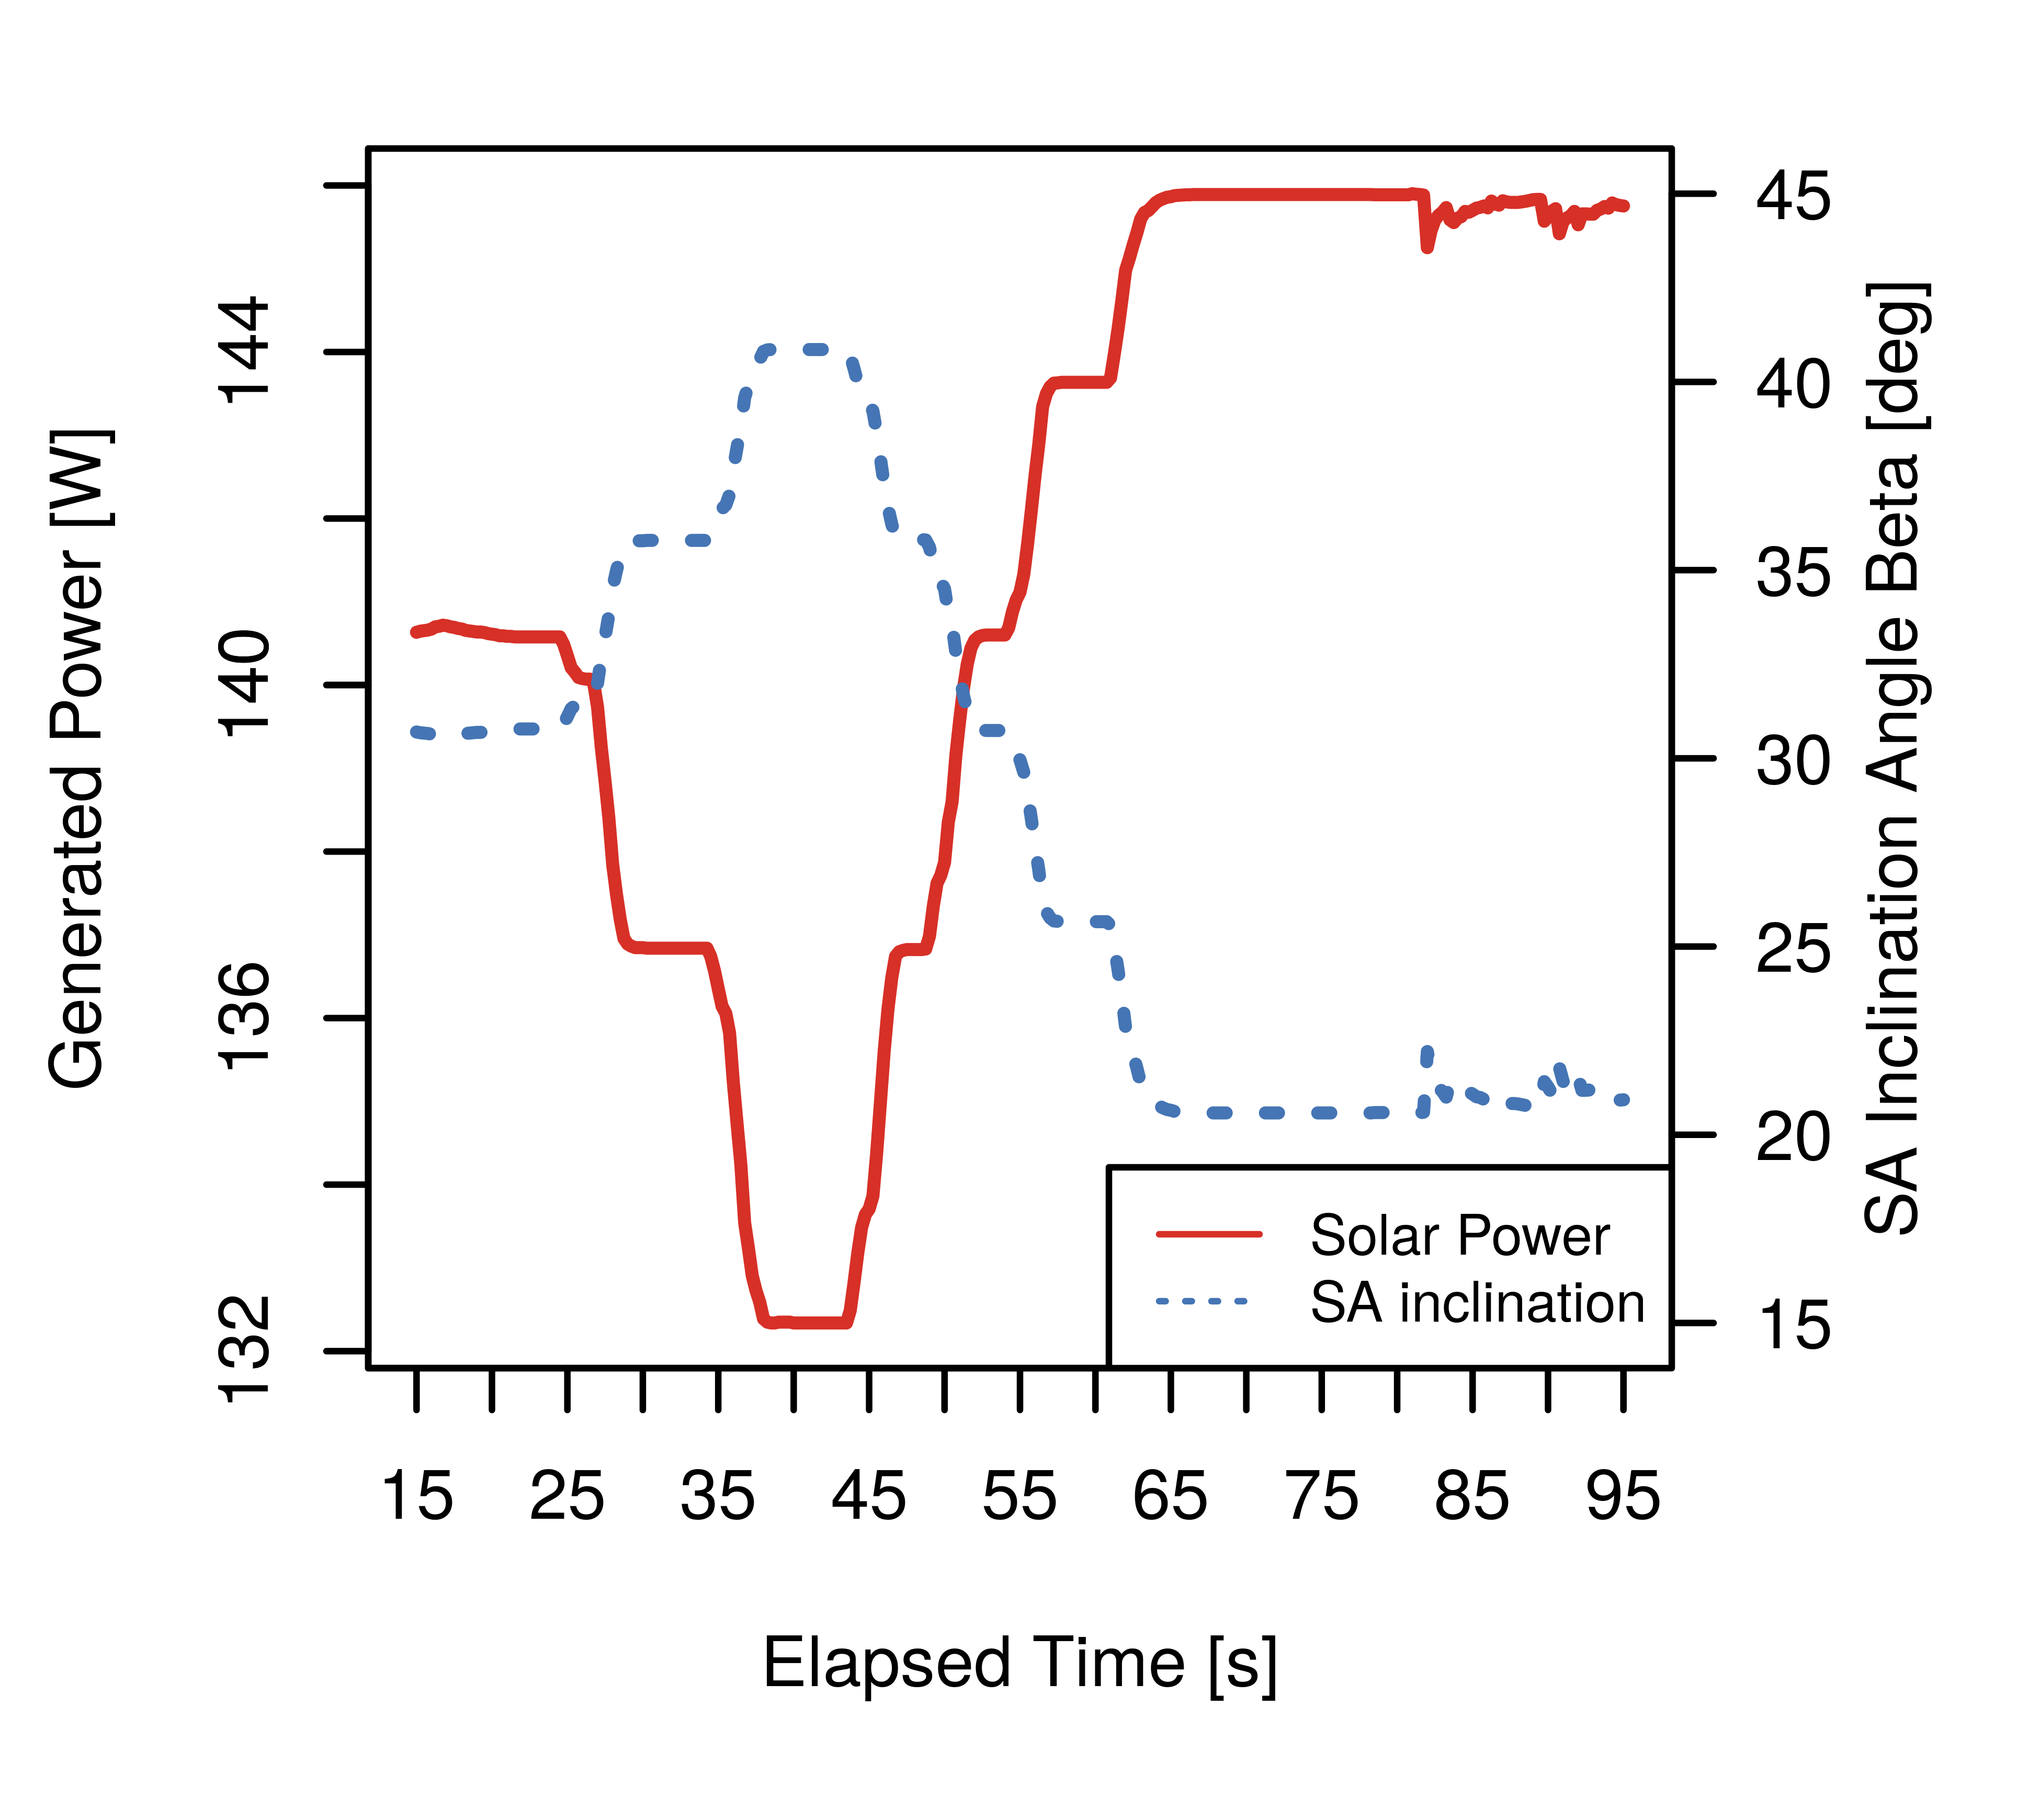
\includegraphics[width=3.25in]{figures/plots/slope-compensation.png}
  \caption{Slope compensation with active suspension system to reduce the \ac{SA} surface inclination angle. Slope inclination angle $B = \SI{30}{\degree}$. In (a), $\beta = B = \SI{30}{\degree}$. In (b), the rover is tilted \SI{10}{\degree} in the opposite direction of the slope so that $\beta = \SI{20}{\degree}$.}
  \label{fig:sub:rover-on-slope-beta}
\end{figure}


%%%%%%%%%%%%%%%%%%%%%%%%%%%%%%%%%%%%%%%%%%%%%
\section{Conclusion}
%%%%%%%%%%%%%%%%%%%%%%%%%%%%%%%%%%%%%%%%%%%%%
The findings of this paper support using the SherpaTT rover active suspension system as a mechanism for solar panel inclination and orientation under certain \ac{SA} sizing conditions. Combining a maximum attainable \ac{SA} surface inclination angle of \SI{10}{\degree} with optimal daily orientation angles results in appreciable traverse gains when compared to what is obtained from a horizontal surface. However, this is not true for large \ac{SA} areas. Furthermore, the smaller the required solar cell coverage area the greater the gains. In light of this, \ac{SA} sizing for the the worst case daily insolations introduce a hibernation mode solar power draw constraint of \SI{17}{\watt} near the equator at \SI{2}{\degree}S and \SI{15}{\watt} in the northern hemisphere at \SI{34}{\degree}N. With these power budgets, an average traverse gain of \SI{34}{\percent} is achieved at \SI{2}{\degree}S for a clear day with a $\tau$ factor of 0.4. At \SI{34}{\degree}N, the average gain is \SI{25}{\percent} under the same atmospheric opacity. These gains remain significant on dusty days at \SI{23}{\percent} and \SI{10}{\percent} at respective latitudes with a $\tau$ factor of 1.

This paper presents an active suspension system use case that goes beyond negotiating complex terrains such as steep slopes or exploring crater environments. The following are a few suggested research topics that expands this idea:

\begin{itemize}
  \item [(1)] Conducting a power budget cost-benefit analysis with respect to the power draws from the suspension systems motors that are required to obtain the sun-facing inclined \ac{SA} surfaces power gains.
  \item [(2)] Achieving higher pitch and rolls angles so that higher \ac{SA} surface inclination angles may be attained.
  \item [(3)] Simulating ground adaption scenarios that preserve a desired \ac{SA} surface position into a fixed plane.
  \item [(4)] Simulating shadowing events on the \ac{SA} and analyzing their affect on power outputs, in particular for shadows caused by the \ac{RA}.
  \item [(5)] Implementing a battery model to simulate battery charge and discharge for a more complete power subsystem simulation.
  \item [(6)] Developing power budgets for onboard instruments to simulate scenarios such as drilling for sample return missions.
  \item [(7)] Proposing SherpaTT \ac{SA} designs for terrestrial and lunar mission scenarios.
  \item [(8)] Exploring other alternative use cases for the rover's active suspension system such as nighttime star tracking for astronomical observations with a mounted telescope.
\end{itemize}


%%%%%%%%%%%%%%%%%%%%%%%%%%%%%%%%%%%%%%%%%%%%%%%%%%%%%%%%%%%%%%%%%%%%%%%%%%%%%%%%%%%%%%%%%%%%%%%%%%%%%%
\bibliographystyle{IEEEtran}
%\bibliography{IEEEabr,MyBibFile}
\begin{thebibliography}{1}

\bibitem{Cordes2018a}
Cordes, F. Design and Experimental Evaluation of a Hybrid Wheeled-Leg Exploration Rover in the Context of Multi-Robot Systems. PhD thesis, University of Bremen. 2018, https://doi.org/10.13140/RG.2.2.24973.79843

\bibitem{Cordes2018b}
Cordes, F, Kirchner, F, Babu, A. Design and field testing of a rover with an actively articulated suspension system in a Mars analog terrain. J Field Robotics. 2018; 35: 1149– 1181. https://doi.org/10.1002/rob.21808

\bibitem{Labreche2020}
Labrèche, G. Exploiting the SherpaTT Rover Active Suspension System to Enable Optimal Solar Array Inclination and Orientation for Long Traverses in a Martian Environment. 2020, http://urn.kb.se/resolve?urn=urn:nbn:se:ltu:diva-78016

\bibitem{Phobos}
DFKI/RIC, Phobos. https://github.com/dfki-ric/phobos. Accessed on: Jun. 12, 2020.

\bibitem{MARSSim}
DFKI/RIC, MARS - Machina Arte Robotum Simulans. https://robotik.dfki-bremen.de/en/research/softwaretools/mars.html. Accessed on: Jun. 12, 2020.

\end{thebibliography}

\end{document}
